\documentclass[a4paper,twoside]{article}


% --- RUIMTE EN LAYOUT ---
\usepackage{setspace}
\setstretch{1.15}

\usepackage{geometry} %size regulating
\geometry{
 a4paper,
 left=25mm,
 right=25mm,
 top=20mm,
 bottom=20mm,
 }

\usepackage{parskip} % for better spacing between paragraphs


% --- WISKUNDE ENSYMBOLEN ---
\usepackage{amsmath, amssymb, amsfonts, amsthm} % For nicer math format
\usepackage{mathrsfs} % For curly arrr
\usepackage{bm} % For bold symbols eg \bm{\nabla}
\usepackage{esint} % For bolletje in integrals
\usepackage{dsfont}
\usepackage{siunitx} % Voeg deze expliciet toe voor die graden en eenheden!


% --- OVERIGE ---

\usepackage{graphicx} % Required for inserting images
\usepackage[hidelinks]{hyperref} % geen kaders om linken
\usepackage{subcaption}
%\usepackage[dutch]{babel}
\usepackage[T1]{fontenc}
\usepackage[utf8]{inputenc}
\usepackage{lmodern}
\usepackage{multicol}

% --- Tikz packages ---
\usepackage{tikz}
\usetikzlibrary{angles,quotes, babel} % for pic (angle labels)
\usetikzlibrary{arrows.meta,decorations.markings,calc, decorations.pathmorphing, decorations.pathreplacing, positioning, shapes, shadings, patterns}
\usepackage{xcolor}
\usepackage{tikz-3dplot}
\usepackage[siunitx]{circuitikz}

\usepackage{etoolbox} % ifthen
\usepackage[outline]{contour} % glow around text
\usepackage{xfp} % higher precision (16 digits?)
\contourlength{1.1pt}



% --- THEOREM STIJLEN MET EXTRA RUIMTE ---

\theoremstyle{definition}
\newtheorem{postulate}{Postulaat}
\newtheorem{definition}{Definitie}
\newtheorem{derivation}{Afleiding}


% --- EXTRA COMMANDO'S ---

\newcommand{\dbar}{{\mkern+3mu\mathchar'26\mkern-12mu d}}

% --- Titel en Introductie --- 

\title{Samenvatting Thermische Fysica}
\author{T. Cools}
\date{Gebaseerd op de hoorcolleges van prof. dr. N. Jachowicz (2025-2026)}

\begin{document}

\maketitle
\hrule
\begin{abstract}
    In deze samenvatting zal per hoofdstuk een overzicht worden gegeven van de belangrijkste concepten, definities, formules, afleidingen en bewijzen die in het vak Thermische Fysica aan bod zijn gekomen.
    De samenvatting is bedoeld voor educatieve doeleinden.
    De samenvatting is gebaseerd op de lessen en cursus van thermische fysica gegeven door prof. dr. N. Jachowicz aan de Universiteit Gent. Alle informatie in deze samenvatting is afkomstig van deze bron, en is bedoeld voor persoonlijk gebruik en studie.
    \medskip
    Auteursrechten: 
    \medskip
    Wat plagiaat betreft, er worden geen letterlijke teksten gekopieerd tenzij er zich af en toe we eens een citaat kan voorkomen, de formuleringen zijn eigen, maar de inhoud is gebaseerd op de cursus. Op algemene titels staan geen auteursrechten, idem geldt voor algemene definities en formules.
    De specifieke formuleringen van de definities, formules en afleidingen (wiskundige stappen) mogen wel, doordat er geen auteursrechten staan op wiskundige logica. Specifieke schetsen of figuren uit de cursus komen dan ook niet voor om de voorgaande redenen. (Eventueel wel eigen figuren.)
\end{abstract}
\hrule

\section{Inleiding}

Het eerste deel van de cursus gaat over de macroscopische beschrijving van de thermische fysica. Dit wil zeggen op grote schaal. Later vanaf hoofdstuk 10 zullen we ook de microscopische beschrijvingen behandelen.
\subsection{Microscopisch en Macroscopisch}

\begin{itemize}
    \item Macroscopisch: 
    
    Behoort tot de klassieke thermodynamica. Hierin worden grootheden zoals druk, volume, temperatuur en energie gebruikt. Deze grootheden zijn gemiddeldes van microscopische grootheden.
    \item Microscopisch:
    
    Behoort tot de statistische mechanica. Hierin worden grootheden zoals de positie en snelheid van individuele deeltjes gebruikt, en ook de individuele eigen energien. Deze grootheden worden vaak achteerhaald met behulp van partitiefuncties en waarschijnlijkheidsverdelingen. 
\end{itemize}

\subsection{Toestanden}

Wanneer een coordinaat evenredig is met de massa, dan is ze \textbf{extensief}, de andere coordinaten zijn \textbf{intensief}. De toestand van een systeem wordt beschreven worden aan de hand van deze coördinaten.

Voorbeeld: Stel we hebben twee bekers water, waarvan de ene een volume van 1 liter heeft en de andere een volume van 2 liter op kamertemperatuur. In dit geval zijn de coördinaten van het systeem de druk, het volume en de temperatuur. 
Het volume is een extensieve grootheid, want wanneer we de 2 bekers samenvoegen, is het nieuwe volume gewoonweg de som van de volumes van de twee bekers. De druk en temperatuur zijn daarentegen intensieve grootheden, want de druk en temperatuur blijven op dat moment hetzelfde als die van de individuele bekers.

Het deel van de ruimte waarin we geïnteresseerd zijn, noemen we het \textbf{systeem}. De rest van de ruimte noemen we de \textbf{omgeving}. Het systeem en de omgeving vormen samen het \textbf{universum}.

\begin{definition}
    \textbf{Geïsoleerd systeem}: Een systeem dat geen energie of stof kan uitwisselen met de omgeving. (geen enkele interactie zoals thermische, mechanische of chemische met de omgeving mogelijk)
\end{definition}

\begin{definition}
    \textbf{Gesloten systeem}: Een systeem dat energie kan uitwisselen met de omgeving, maar geen stof kan uitwisselen.
\end{definition}

\begin{definition}
    \textbf{Diathermische wand}: Een wand die warmte kan doorlaten, maar geen materie. (laat alleen thermiche interacties toe)
\end{definition}

\begin{definition}
    \textbf{Adiabatische wand}: Een wand die geen warmte kan doorlaten (geen thermische interacties), maar de wand kan wel verplaatst worden (laat alleen mechanische interacties toe), de wand kan ook materie doorlaten, maar is niet per se nodig.
\end{definition}

Verschillende soorten interacties:
\begin{itemize}
    \item Mechanische interacties (vaste wanden \(\implies\) geen mechanische enrgie-uitwisseling, beweegbare wanden \(\implies\) wel mechanische energie-uitwisseling)
    \item Thermische interacties (adiabatische wanden \(\implies\) geen thermische interacties, diathermische wanden \(\implies\) wel thermische interacties)
    \item Chemische interacties (wanden die materie kunnen doorlaten \(\implies\) chemische interacties, wanden die geen materie kunnen doorlaten \(\implies\) geen chemische interacties)
\end{itemize}

\begin{definition}
    \textbf{Thermodynamisch evenwicht}: Systeem  als teglijkertijd mechanisch, thermisch en chemisch evenwicht is.
\end{definition}

\begin{definition}
  \textbf{Thermodynamische processen}: Veranderingen in de toestand van een systeem. Er zijn verschillende soorten processen, zoals isotherm (temperatuur blijft constant), isobaar (druk blijft constant), isochorisch (volume blijft constant) en adiabatisch (geen warmte-uitwisseling).  
\end{definition}

Als processen langzaam genoeg verlopen, kunnen we aannemen dat het systeem zich in een evenwichtstoestand bevindt tijdens het hele proces. We noemen dit een \textbf{quasi-statisch proces}.

De tijd om op evenwicht te komen, noemen we de \textbf{relaxatietijd} \(t_R\). (Dit komt niet meer aan bod verder dan hier)



\section{Temperatuur en Thermisch evenwicht}

\subsection{Temperatuur en Thermometers}

Dit stuk is vooral een kwalitatieve beschrijving, maar ook te kennen!

De eerste thermometer was een bimetalen strip waarbij het ene metaal meer uitzet dan het andere bij verwarming, waardoor de strip kromt. De kromming van de strip kan worden gebruikt om de temperatuur te meten. (toepassingen in ovens of als uitschakelaars voor bv een koffiezetapparaat)
Later werden ook thermokoppels gebruikt, waarbij twee verschillende metalen aan elkaar worden verbonden. Wanneer er een temperatuurverschil is tussen de twee metalen, ontstaat er een elektrische spanning (ems) die kan worden gemeten en omgezet in een temperatuurwaarde. Wel is er een referentiepunt nodig zoals vloeibare stikstof in evenwicht met damp.

We hebben ook nog weerstandstermometers, waarbij de elektrische weerstand van een materiaal verandert met de temperatuur. Door de weerstand te meten, kan de temperatuur worden bepaald. Vaak wordt platina als dunne metaaldraad gebruikt die tot een spoel wordt gewikkeld.

Voor hoge temperaturen worden pyrometers of optische thermometers gebruikt, die de stralingsintensiteit van een object meten \footnote{stralingswet van planck zie vb H12 voor afleiding}. De intensiteit van de straling is gerelateerd aan de temperatuur van het object volgens de wet van Planck.
De werking van een pyrometer is gebaseerd op de vergeelijking van de helderheid van een object en van een gloeidraad. De temperatuur van het object kan worden bepaald door de helderheid van het object te vergelijken met die van een gloeidraad waarvan de temperatuur bekend is. De gloeidraad wordt verwarmd totdat de helderheid overeenkomt met die van het object, en de temperatuur van de gloeidraad wordt dan als de temperatuur van het object beschouwd.  

Nadeel: Het bereik is beperkt door gebruikte kleurenfilters en de maximale temperatuur van de gloeidraad.

\subsection{Nulde wet Thermodynamica}

Wanneer twee systemen in thermisch contact worden gebracht, dan streven ze naar dezelfde temperatuur. Als deze temperatuur is bereikt, zijn de systemen in \textbf{Thermisch evenwicht}. 
Twee systemen zijn in thermisch evenwicht als er geen netto warmteoverdracht plaatsvindt tussen de systemen.

\begin{postulate}
\textbf{Nulde wet van de thermodynamica}: Als twee systemen in thermisch evenwicht zijn met een derde systeem, dan zijn ze ook in thermisch evenwicht met elkaar.
\end{postulate}

Stel, systeem A is in thermisch evenwicht met systeem C, en systeem B is ook in thermisch evenwicht met systeem C. Volgens de nulde wet van de thermodynamica, zijn systemen A en B ook in thermisch evenwicht met elkaar. 

\begin{definition}
    \textbf{Een isotherm}: De verzameling van punten die alle toestanden waarvoor een systeem in thermisch evenwicht is met een bepaald referentiesysteem voorstellen.
\end{definition}

\begin{definition}
    \textbf{Temperatuur}: De temperatuur van een systeem is een grootheid die bepaald of het systeem al dan niet in thermisch evenwicht is met andere systemen.
\end{definition}

\begin{definition}
    \textbf{Empirische temperaturen}: Temperatuurmetingen gebaseerd op evenwichtstoestanden van een thermodynamisch systeem.
    De temperaturen worden gedefinieerd via een meetbare eigenschap die monotoon veranderd met hoe warm/koud een systeem is zonder dat je al een absolute energiemaatstaf of kelvinschaal nodig hebt.
\end{definition}

\subsection{Temperatuurschalen}

De Belangrijkste schaal is de absolute temperatuurschaal of de \textbf{Kelvinschaal}, waarbij het absolute nulpunt (0 K) overeenkomt met de laagst mogelijke temperatuur.

Van Celcius naar Fahrenheit: 

tussen 0 en 100 gradeen zijn er 100 intervallen voor celcius een 180 inntervallen voor fahrenheit, dus 1 graad celcius komt overeen met $\frac{180}{100} = \frac{9}{5}$ graden fahrenheit. Daarnaast is er een verschil van 32 graden tussen de twee schalen bij het nulpunt van celcius, dus de formule voor het omrekenen van Fahrenheit naar Celcius is:

\(T(^\circ C) = \frac{5}{9}T(^\circ F) - 32\)

Van Celcius naar Kelvin: \(T(K) = T(^\circ C) + 273.15\) wat triviaal is.

De waarschijnlijk bekendste thermometer is de kwikthermometer, waarbij de uitzetting van kwik wordt gebruikt om de temperatuur te meten. De schaalverdeling op de thermometer is gebaseerd op het vriespunt (0 °C) en het kookpunt (100 °C) van water bij standaarddruk.

Er zijn 2 vaste punten nodig om de schaal in te stellen. We nemen voor de eerste \(P=0\) bij \(T=0\), voor het tweede vast punt wordt het \textbf{tripelpunt} \footnote{Punt waar de 3 weelgekende fases samen in evenwicht bestaan} van water genomen. Dit gebeurd bij \(T = 273.16 K\) en \(P=611.73\)Pa.
We kunnen nu de schaal instellen door deze twee punten te verbinden met een rechte lijn, waarbij we de temperatuur van het tweede punt op 273,16 K zetten. 

De absolute temperatuur wordt:
\[
T = (273,16 K)\left( \frac{P}{P_{tp}} \right)
\]
waarbij \(P_{tp}\) de druk is bij het tripelpunt van water, en \(P\) de druk op het moment van tempertatuur \(T\).

Absolute temperatuurschaal:
\[
T =(273,16 K) \lim_{P \to P_{tp}} \left( \frac{P}{P_{tp}} \right)
\]

Hier moeten we de bijzondere eigenschap onthouden dat voor deze extrapolatie van deze metingen voor verschillende gassen naar een verdwijnende druk \(P_{tp}\) altijd dezelfde waarde van \(T\) oplevert, namelijk 273,16 K.
Ik dacht dat dit de limiet was waar het gedrag van een algemeen gas steeds meer op dat van een ideaal gas lijkt, maar dit ben ik niet zeker.
\section{Eenvoudige thermodynamische systemen}
\subsection{PV-diagrammen (zuivere stof)}
\begin{figure}[htp]
    \centering
    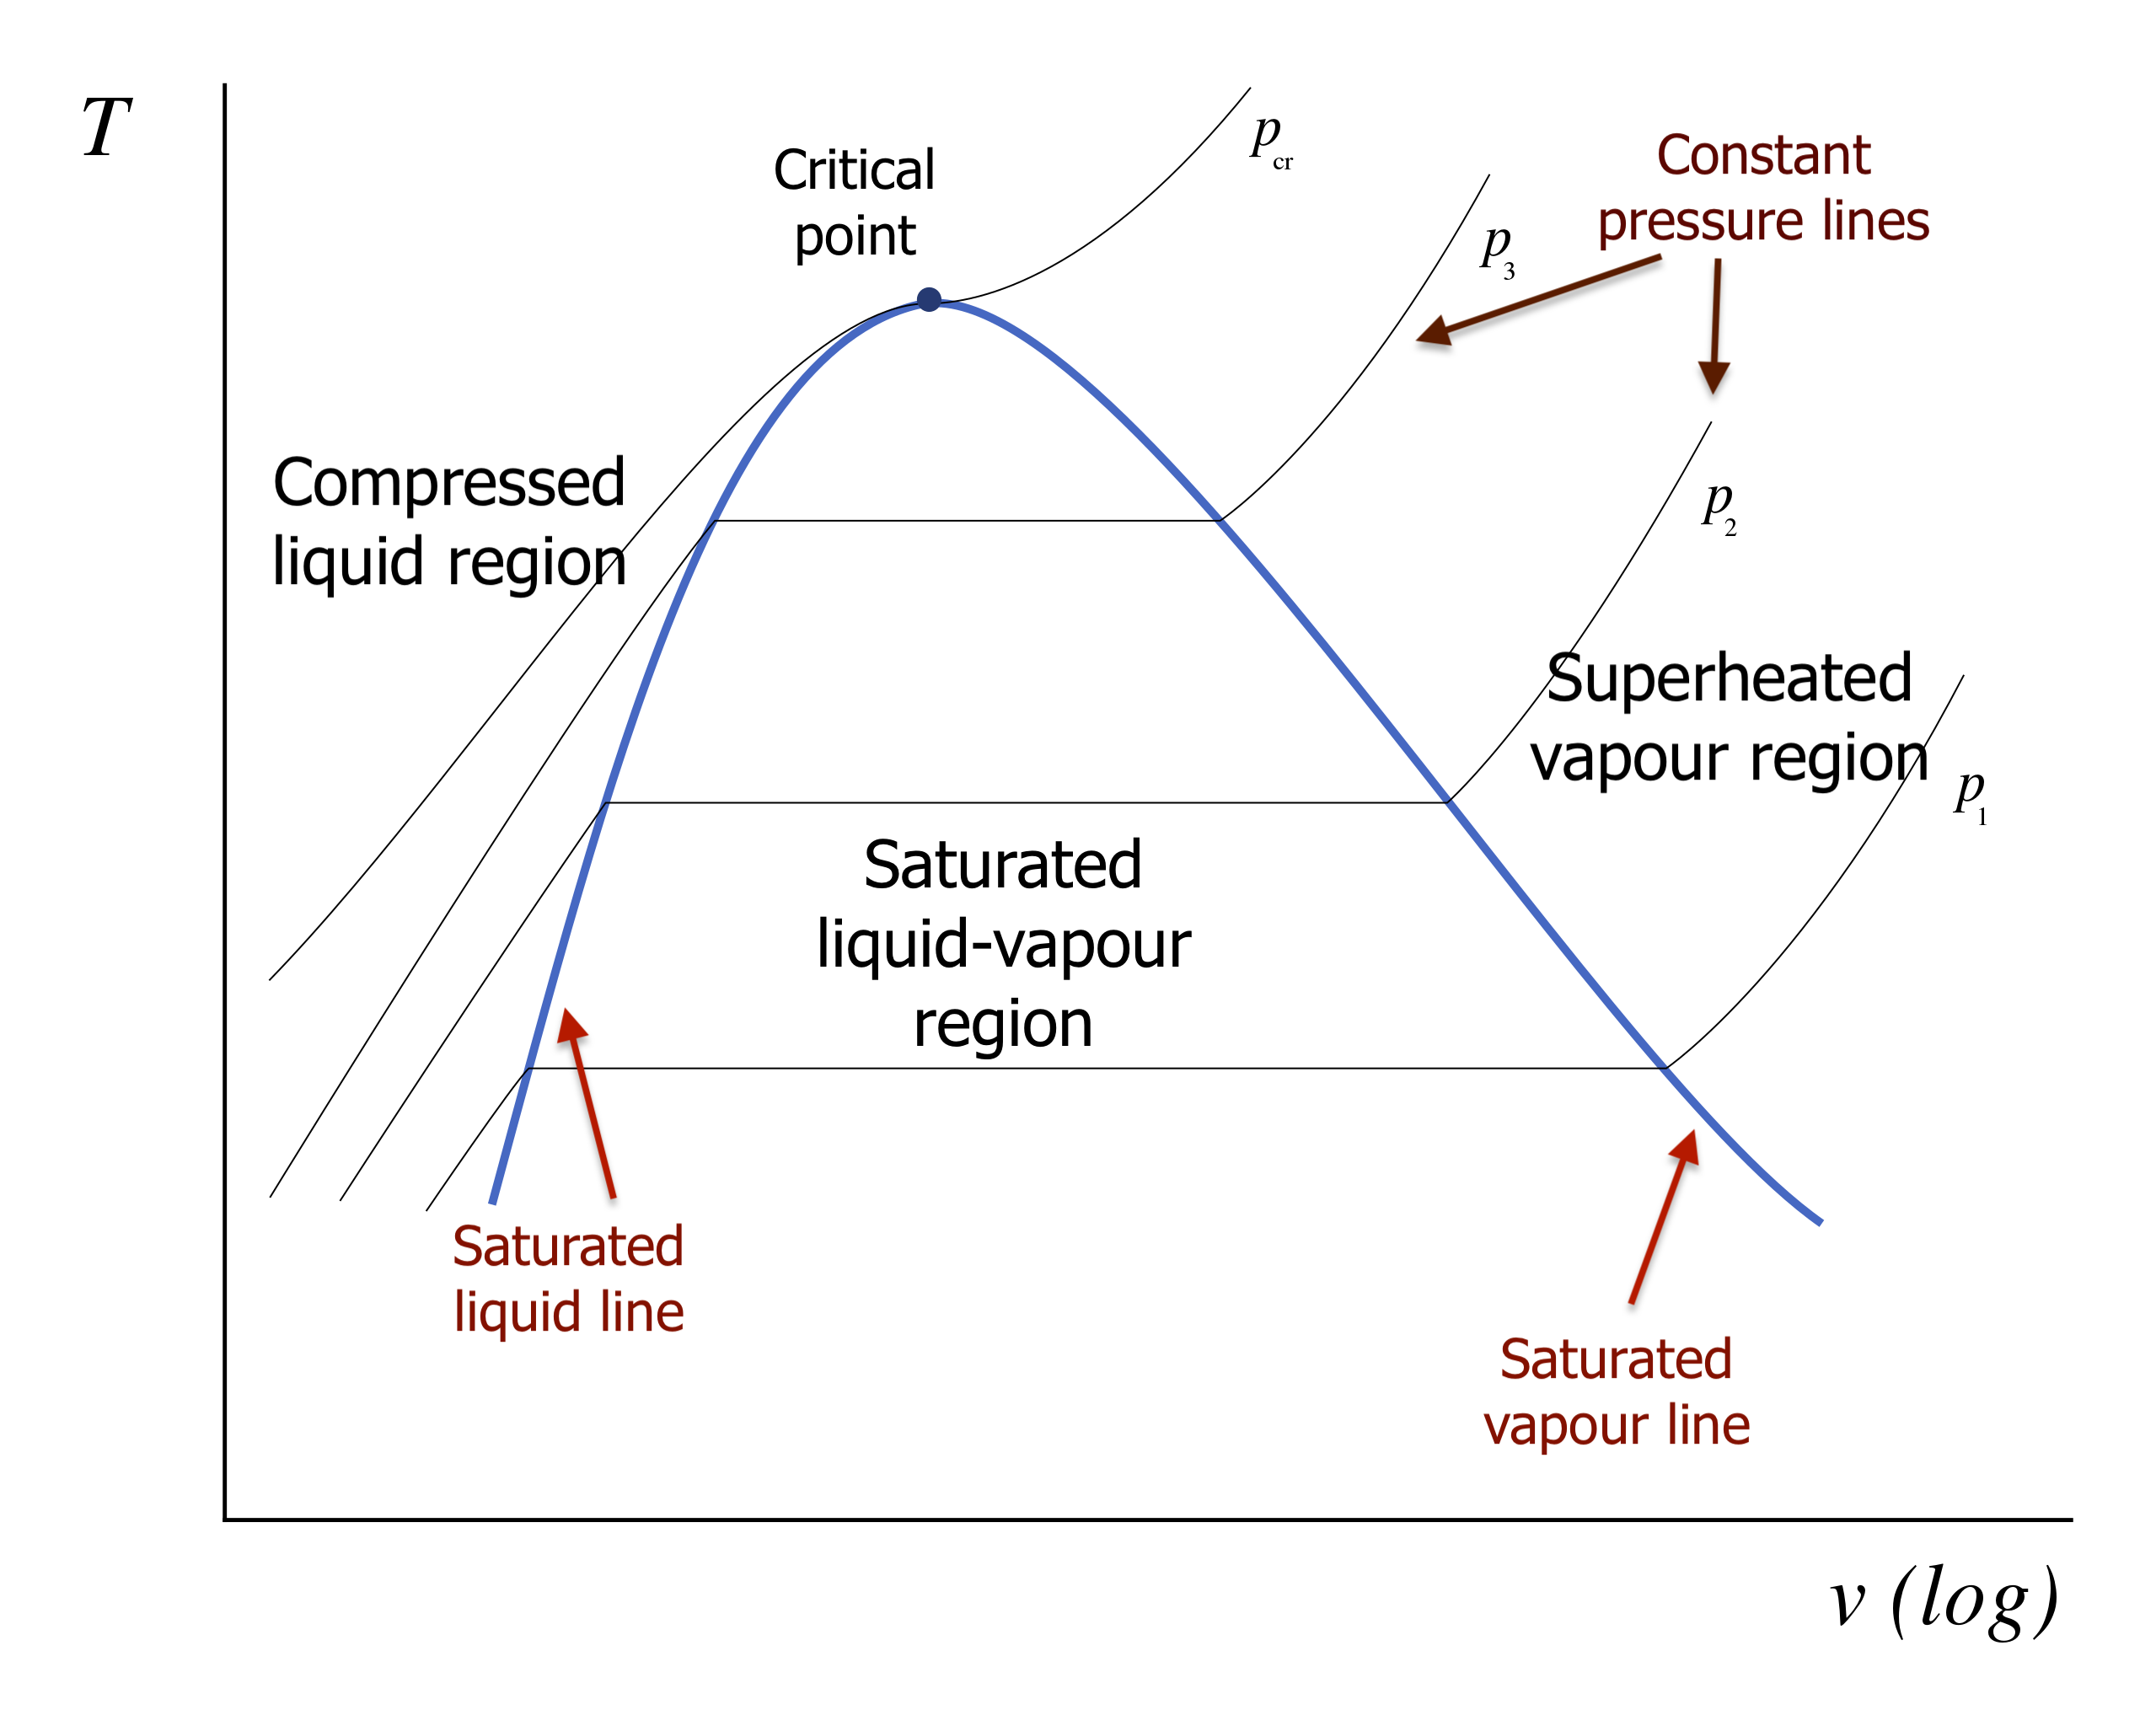
\includegraphics[width=0.5\textwidth]{Foto's-Figuren/Fig.-2-8_T-v_diagram_for_a_liquid_vapor-copy.svg_.png}
    \caption{VT-diagram van een zuivere stof. De verschillende lijnen en gebieden geven de verschillende fasen en evenwichten aan. \footnotesize \copyright{Olivier Cleynen is licensed under a CC0 (Creative Commons Zero) license}}
    \label{fig:VT-diagram}
\end{figure}
\begin{figure}
    \centering
    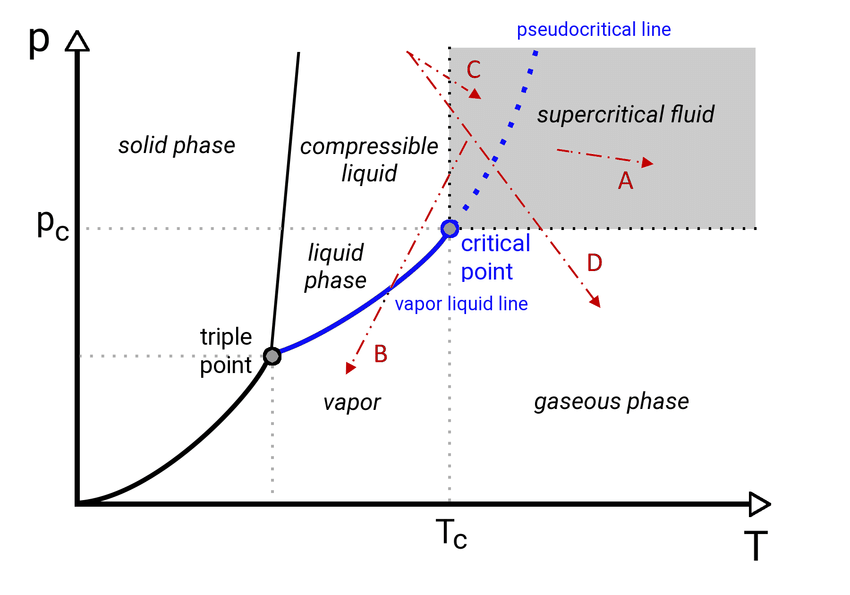
\includegraphics[width=0.5\textwidth]{Foto's-Figuren/P-T-diagram-Supercritical-fluid-region-and-various-supercritical-injection-types.ppm.png}
    \caption{PT-diagram van een zuivere stof. De verschillende lijnen en gebieden geven de verschillende fasen en evenwichten aan 
        \footnotesize \textcopyright{SUPERCRITICAL AND TRANSCRITICAL TURBULENT INJECTION PROCESSES: CONSISTENCY OF NUMERICAL MODELING - Scientific Figure on ResearchGate. Available from: \url{https://www.researchgate.net/figure/P-T-diagram-Supercritical-fluid-region-and-various-supercritical-injection-types_fig1_349274264} [accessed 10 May 2026]}}
    \label{fig:PT-diagram}
\end{figure}

\begin{figure}
    \centering
    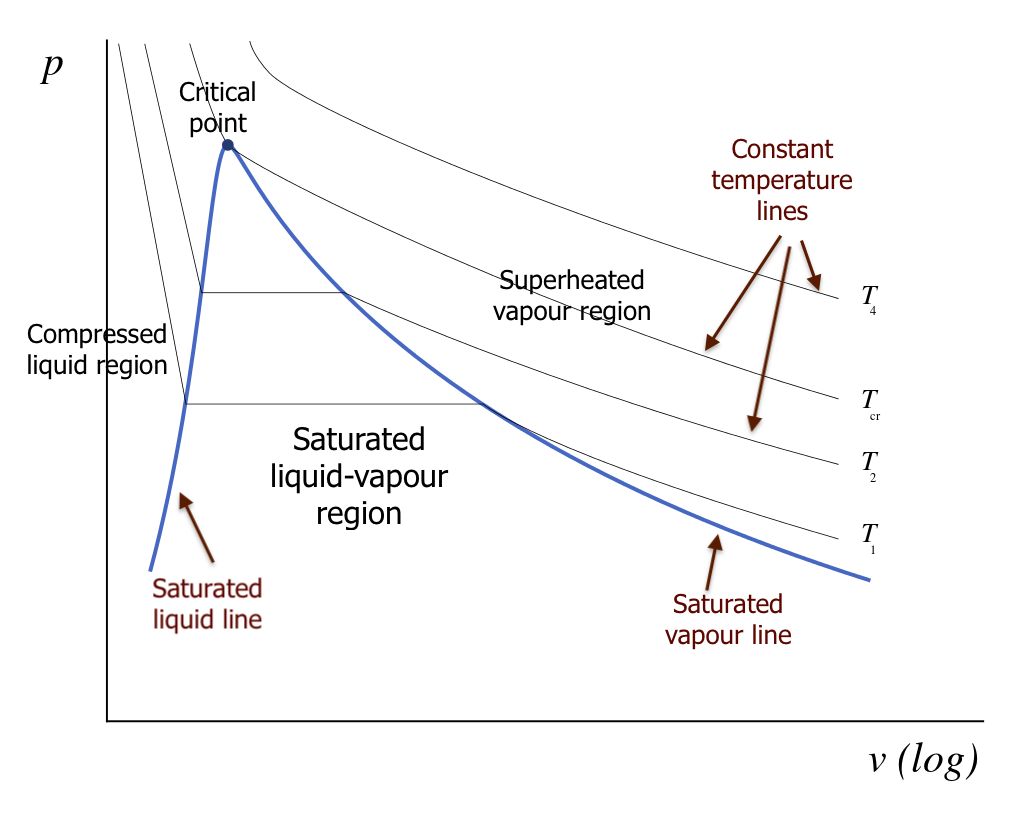
\includegraphics[width=0.5\textwidth]{Foto's-Figuren/Fig-2-9_P-v_diagram_for_a_liquid-vapor.svg_.png}
    \caption{PV-diagram van water. De verschillende lijnen en gebieden geven de verschillende fasen en evenwichten aan. \footnotesize \copyright{Olivier Cleynen is licensed under a CC0 (Creative Commons Zero) license}}
    \label{fig:PV-diagram}
\end{figure}

\begin{definition}
    \textbf{Vloeistofverzadigingslijn}: De lijn in een PV-diagram waarbij vloeistof en damp in evenwicht zijn. Deze lijn scheidt het gebied van de vloeistoftoestanden van het gebied van de damp-toestanden.
\end{definition}
\medskip
\begin{definition}
    \textbf{Kritische temperatuur}: De temperatuur waarbij de vloeistofverzadigingslijn eindigt. Boven deze temperatuur kunnen vloeistof en damp niet meer in evenwicht zijn, en is er geen onderscheid meer tussen de twee fasen.
\end{definition}
\medskip
\begin{definition}
    \textbf{Kritische isotherm}: De isotherm die door het kritische punt gaat. Deze isotherm heeft een horizontaal inflectiepunt bij het kritische punt, wat betekent dat de eerste en tweede afgeleide van de druk naar het volume gelijk zijn aan nul op dat punt.
\end{definition}
\medskip
\begin{definition}
    \textbf{Kritisch punt K}: Het punt in het PV-diagram waar de vloeistofverzadigingslijn eindigt. Op dit punt zijn de eigenschappen van de vloeistof en de damp identiek, en er is geen onderscheid meer tussen de twee fasen.
\end{definition}
\medskip
\begin{definition}
    \textbf{Kritische druk}: De druk die overeenkomt met het kritische punt in het PV-diagram. Dit is de druk waarbij de vloeistofverzadigingslijn eindigt en de kritische isotherm een horizontaal inflectiepunt heeft.
\end{definition}
\medskip
\begin{definition}
    \textbf{Verzadigde vloeistof}: Een vloeistof die in evenwicht is met haar eigen damp. Deze vloeistof heeft een constante druk en temperatuur.
\end{definition}
\medskip
\begin{definition}
    \textbf{Verzadigde damp}: Een damp die in evenwicht is met zijn eigen vloeistof. Deze damp heeft een constante druk en temperatuur.
\end{definition}
\medskip
\begin{definition}
    \textbf{Dampverzadigingslijn}: De lijn in een PV-diagram waarbij damp en vloeistof in evenwicht zijn. Deze lijn scheidt het gebied van de damp-toestanden van het gebied van de vloeistoftoestanden.
\end{definition}
\medskip
De dampverzadigingslijn en de vloeistofverzadigingslijn ontmoeten elkaar bij het kritische punt K, waar de eigenschappen van de vloeistof en de damp identiek zijn.

\begin{definition}
    \textbf{Tripellijn}: De lijn in een PV-diagram waarbij de vloeistof-damp en vaste-stof-damp in evenwicht zijn. (Dus nog niet perse de vloeibare fase inbegrepen)
\end{definition}
\subsection{PT-diagrammen (zuivere stof)}
\begin{definition}
    \textbf{Tripelpunt}: Het punt in een PV(T)-diagram waar de drie fasen van een stof in evenwicht zijn. Op dit punt kunnen alle drie de fasen tegelijkertijd bestaan. Dit punt ligt op de tripellijn van het Pv-diagram.
\end{definition}
\medskip
\begin{definition}
    \textbf{Sublimatielijn}: De lijn in een PT-diagram waarbij de vaste stof en de damp in evenwicht zijn. Deze lijn scheidt het gebied van de vaste-stof-toestanden van het gebied van de damp-toestanden.
\end{definition}
\medskip
\begin{definition}
    \textbf{Verdampingslijn}: De lijn in een PT-diagram waarbij de vloeistof en de damp in evenwicht zijn. Deze lijn scheidt het gebied van de vloeistoftoestanden van het gebied van de damp-toestanden.
\end{definition}
\medskip
\begin{definition}
    \textbf{Stollingslijn}: De lijn in een PT-diagram waarbij de vaste stof en de vloeistof in evenwicht zijn. Deze lijn scheidt het gebied van de vaste-stof-toestanden van het gebied van de vloeistoftoestanden.
\end{definition}
De drie scheidingslijnen (sublimatielijn, verdampingslijn en stollingslijn) ontmoeten elkaar bij het tripelpunt, waar alle drie de fasen in evenwicht zijn.
De helling van de sublimatielijn en verdampingslijn is altijd positief, terwijl de helling van de stollingslijn kan variëren afhankelijk van de stof.
Voor water heeft de stollingslijn een negatieve helling, wat betekent dat de smelttemperatuur van water afneemt met toenemende druk.
Voor de meeste andere stoffen heeft de stollingslijn een positieve helling, wat betekent dat de smelttemperatuur toeneemt met toenemende druk.

\subsection{Het PVT-opprevlak}
Het is belangrijk dat je deze 3D diagrammen goed kan interpreteren, en dat je weet wat de verschillende lijnen en vlakken betekenen en ze kan uitleggeen aan de hand van voorgaande definities.

\begin{figure}[h]
    \centering
    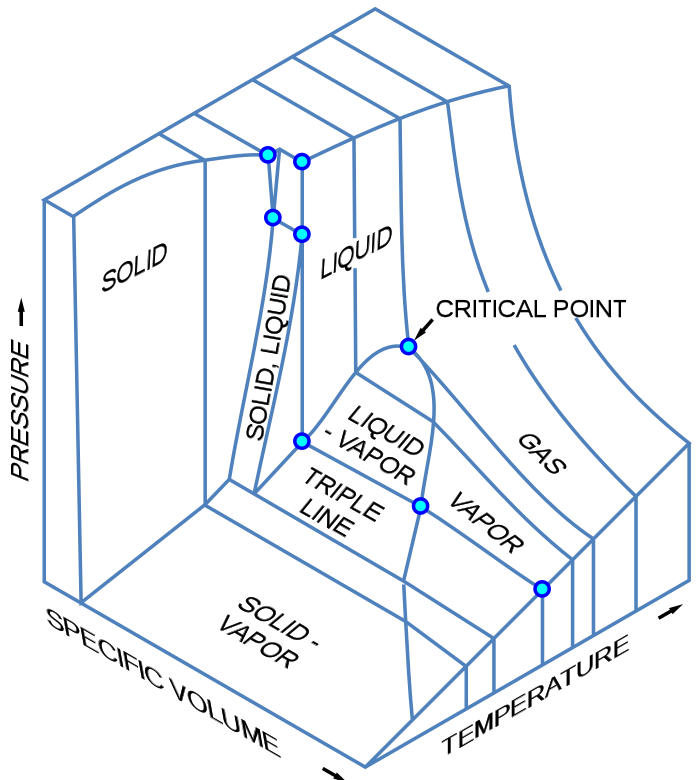
\includegraphics[width=0.5\textwidth]{Foto's-Figuren/Fig.-2-6-1.png}
    \caption{PVT-diagram van een zuivere stof. De verschillende lijnen en gebieden geven de verschillende fasen en evenwichten aan.\footnotesize \copyright{ vectorization is licensed under a CC0 (Creative Commons Zero) license.}}
    \label{fig:PVT-diagram}
\end{figure}


\subsection{Toestandsvergelijkingen}

De toestandsvergelijking:
\[ f(P,V,T) = 0 \]
is een vergelijking die de relatie tussen druk, volume en temperatuur van een stof beschrijft.
Voor een ideaal gas is deze vergelijking \(PV = nRT\), maar voor reële gassen kunnen er afwijkingen zijn van deze eenvoudige relatie, en kunnen er meer complexe toestandsvergelijkingen worden gebruikt, zoals de van der Waals vergelijking \footnote{Deze  is gebaseerd op de kinetische gastheorie in hoofdstuk 10.}.

Het bijzondere aan deze toestandsfuncties is dat wanneer we twee coordniiaten vast nemen, de derde coordinaat automatisch ook vast ligt. Er zijin dus slechts twee coordinaten onafhankelijk!

\subsection{Differentiële toestandsvergelijkingen}

\begin{postulate}
    Iedere infinitesimale verandering in de thermodynamica moet aan de voorwaarde voldoen dat deee verandering van grootheid die zodanig klein is tegenover de grootheid zelf, dat we kunnen zeggen dat de verandering van grootheid oneindig klein is.
\end{postulate}

Dit is een continuïteitsvoorwaarde die ervoor zorgt dat we kunnen werken met differentiaalvergelijkingen in plaats van discrete veranderingen.

Hierdoor kan V geschreven worden als \(V = V(T,P)\) en kunnen we de totale differentiaal van V schrijven als:
\[dV = \left( \frac{\partial V}{\partial T} \right)_P dT + \left( \frac{\partial V}{\partial P} \right)_T dP\]

Bij constante druk \(dP = 0\), definieren we de \textbf{volume-uitzettingscoëfficiënt}:
\begin{equation}
    \label{eq: volume-uitzettingscoefficient}
    \beta = \frac{1}{V} \left( \frac{\partial V}{\partial T} \right)_P
\end{equation}
Waarbij de \(\frac{1}{V}\) de normering voor het volume is. (Als V verdubbelt, verdubbelt ook de uitzetting, dus we moeten dit normeren.)

Bij constante temperatuur \(dT = 0\), definieren we de \textbf{isothermische drukbaarheid}:
\begin{equation}
    \label{eq:isothermische-drukbaarheid}
    \kappa = -\frac{1}{V} \left( \frac{\partial V}{\partial P} \right)_T
\end{equation}
Waarbij het minteken zorgt voor een positieve waarde voor \(\kappa\), aangezien het volume afneemt met toenemende druk. De \(\frac{1}{V}\) term is opnieuw de normering voor het volume.
Deze waarde is vooral belangrijk voor gasssen, omdat gassen veel samendrukbaar zijn, terwijl vloeistoffen en vaste stoffen veel minder samendrukbaar zijn.

We kunnen hetzelfde doen voor de totale differentialen van\(P(V,T)\) en \(T(P,V)\):
\[dP = \left( \frac{\partial P}{\partial V} \right)_T dV + \left( \frac{\partial P}{\partial T} \right)_V dT\]
\[dT = \left( \frac{\partial T}{\partial P} \right)_V dP + \left( \frac{\partial T}{\partial V} \right)_P dV\]

We kunnen \(dP\) ook uitdrukken in termen van \(\beta\) en \(\kappa\) door de totale differentiaal van \(V(T,P)\) te gebruiken:
\[dV = V \beta dT - V \kappa dP\]
\[dP = \frac{\beta}{\kappa} dT - \frac{1}{V \kappa} dV\]

\subsection{Thermodynamische systemen}
De methodiek van deze systemen is dat we steeds een extensieve grootheid (een veralgemeende verplaatsing) hebben en twee intensieve grootheden waarvan 1 steeds de temparatuur is en de andere een veralgemeende kracht.
We kunnen dan toestandsfuncties schrijven in termen van deze grootheden, en we kunnen ook differentiaalvergelijkingen schrijven voor deze toestandsfuncties. 
\subsubsection{Gespannen snaar}
Onze drie coordinaten zijn hier de temperatuur \(T\), de kracht \(F\) en de lengte \(L\). De extensieve grootheid is hier de lengte \(L\), en de intensieve grootheden zijn de temperatuur \(T\) en de kracht \(F\).

De wet van hook zegt:
\[F = k \Delta L\]
waarbij \(k\) de veerconstante is, en \(\Delta L\) de verandering in lengte is ten opzichte van de onbelaste lengte \(L_0\).

De totale differentiaal van \(L=L(T,F)\) is:
\[dL = \left( \frac{\partial L}{\partial T} \right)_F dT + \left( \frac{\partial L}{\partial F} \right)_T dF\]
We kunnen de lengte-uitzettingscoëfficiënt, definiëren:
\begin{equation}
    \label{eq: lengte-uitzettingscoefficient}
    \alpha = \frac{1}{L} \left( \frac{\partial L}{\partial T} \right)_F
\end{equation}
en de elasticiteitsmodulus \(Y\):
\begin{equation}
    \label{eq: elasticiteitsmodulus}
    Y =  \frac{L}{A}\left( \frac{\partial F}{\partial L} \right)_T
\end{equation}
met A de doorsnede. De voorfactoren zorgen ervoor dat deze grootheden genormaliseerd zijn, zodat ze niet afhankelijk zijn van de grootte van het systeem.

In deze situatie wordt de volume-uitzettingscoëfficiënt \(\beta\) herschreven als:
\[\beta = \frac{1}{V} \left( \frac{\partial V}{\partial T} \right)_F = \frac{1}{L_1L_2L_3} \left( L_2L_3\frac{\partial L_1}{\partial T} + L_1L_3\frac{\partial L_2}{\partial T} + L_1L_2\frac{\partial L_3}{\partial T} \right)_F \]
Doordat we naar 1 dezelfde materiaal kijken is de lineaire-uitzettingscoëfficiënt voor alle lengtes hetzelfde, dus kunnen we dit herschrijven als:
\[\beta =  \frac{1}{L_1}\left(\frac{\partial L_1}{\partial T}\right)_F + \frac{1}{L_2}\left(\frac{\partial L_2}{\partial T}\right)_F + \frac{1}{L_3}\left(\frac{\partial L_3}{\partial T}\right)_F  = 3 \alpha\]

\subsubsection{Oppervlaktefilms}

3 categorieën van oppervlaktefilms:
\begin{itemize}
    \item Vloeistofoppervlakte: De oppervlakte van een vloeistof in contact met een gas. 
    \item Vloeistof-vloeistofoppervlakte: De oppervlakte van een vloeistof in contact met een andere vloeistof.
    \item De oppervlakte van een zeepbel die in contact is met een gas aan beide kanten.
\end{itemize}   

De grootheden zijn hier de temperatuur \(T\) (intensief), de oppervlakte \(A\) (extensief) en de oppervlaktespanning \(\gamma\) (intensief).

\textbf{oppervlaktespanning} \(\gamma\):
\[\gamma = \frac{F}{l}\]
Als het oppervlak aan 2 kanten is, dan is de oppervlaktespanning (voor bv een zeepbel):
\[\gamma = \frac{F}{2l}\]

Zuivere vloeistof in evenwicht met damp:
\[\gamma = \gamma_0 \left(1 - \frac{T}{T'_c}\right)^{n}\]
waarbij \(\gamma_0\) de oppervlaktespanning bij 0 K is, \(T'_c\) de bijna kritische temperatuur is, en \(n\) een exponent is die afhangt van de specifieke vloeistof (meestal tussen 1 en 2).
Deze formule geeft aan dat de oppervlaktespanning afneemt naarmate de temperatuur stijgt, en dat ze nul wordt bij de kritische temperatuur, waar er geen onderscheid meer is tussen vloeistof en damp.

Voor een monomoleculaire oppervlaktefilm op water binnen bepaalde grenzen van oppervlakte \(A\):
\[(\gamma-\gamma_w)A = cst T\]
waarbij \(\gamma_w\) de oppervlaktespanning van het water is, en \(cst\) een constante die afhangt van de specifieke film.

\textbf{Oppervlaktedruk}: \(\gamma-\gamma_w\)

\subsubsection{Elektrolytische cel}

De elektrolytische cel is een elektrochemische cel die reversibel is. Voor verdere details verwijs ik jullie naar de cursus van chemie.

De wet van Faraday zegt:
\[\Delta Z = \Delta n j N_F\]
waarbij \(\Delta Z\) het verschil in elektrische lading is die door de cel stroomt,\(\Delta n\) het verschil aantal mol elektronen is dat wordt overgedragen in de redoxreactie, j de valentie elekronen per reactie zijn, en \(N_F\) de Faraday-constante is, die gelijk is aan de lading van één mol elektronen (ongeveer 96485 coulomb per mol).


De drie coordinaten zijn hier de temperatuur \(T\) (intensief), de elektrische potentiaal \(V_\epsilon\) (intensief) en de lading \(Z\) (extensief).

De toestandsvergelijking van een verzadigde reversibele cel is:
\[V_\epsilon = V_{\epsilon,25} + \alpha (T'-25^\circ C) + \beta (T'-25^\circ C)^2 + \gamma (T' - 25^\circ C)^3\]

waarbij \(V_{\epsilon,25}\) de elektrische potentiaal is bij 25 °C, en \(\alpha\), \(\beta\) en \(\gamma\) empirische constanten zijn, dus niet de coëfficienten van eerder.

\subsubsection{Diëlektricum}

De theorie van diëlektrica zou gekend moeten zijn van elektriciteit een magnetisme en relativeit \& elektromagnetisme.
De diëlektrische verplaatsing \(D\):
\[D = \epsilon_0 E  + P = \epsilon_0 E + \frac{\Pi}{V}\]
waarbij \(\epsilon_0\) de permittiviteit van het vacuüm is, \(E\) het elektrische veld is, \(P\) de polarisatie is, \(\epsilon_0\) de permittiviteit van het vacuüm is, en \(\Pi\) de totale dipoolmoment is.

De drie grootheden zijn hier de temperatuur \(T\) (intensief), het elektrische veld \(E\) (intensief) en de totale dipoolmoment \(\Pi\) (extensief).

Met een toestandsvergelijking van de vorm:
\[\frac{\Pi}{V} = \left(a + \frac{b}{T} \right)\]
met a en b constanten die afhangen van het diëlektricum.

\subsubsection{Paramagnetische staaf}

De drie grootheden zijn hier de temperatuur \(T\) (intensief), het magnetisch veld \(H\) (intensief) en de magnetische moment \(M\) (extensief).
\footnote{Let op, in andere cursussen heten \(H\) of \(B\) het magnetisch veld wegens historische verwarring}

De magnetische inductie \(B\) is gerelateerd aan het magnetisch veld \(H\) en de magnetisatie \(M\) door de relatie:
\[B = \mu_0 (H + \frac{M}{V})\]
waarbij \(\mu_0\) de permeabiliteit van het vacuüm is.

We hebben de toestandsvergelijking:
\[M = \frac{C_c}{T} H\]
waarbij \(C_c\) de Curie-constante is, die afhangt van het materiaal van de paramagnetische staaf.

\subsubsection{Toestandsvergelijking van een gas }

\textbf{Viriaalontwikkeling}:
\[\frac{PV}{nRT} = 1 + \frac{B(T)}{V} + \frac{C(T)}{V^2} + \ldots = Z\]
waarbij \(B(T)\) en \(C(T)\) de viriale coëfficiënten zijn, die afhangen van de temperatuur en de specifieke eigenschappen van het gas. Deze coëfficiënten corrigeren voor de interacties tussen de gasmoleculen, waardoor de vergelijking nauwkeuriger wordt voor reële gassen bij hogere drukken en lagere temperaturen.
\(Z\) is de compressiefactor, die aangeeft hoe ver het gas afwijkt van het ideale gasgedrag. Voor een ideaal gas is \(Z = 1\).

Voor ideale gassen bij constante deeltjes gelden de volgende drie wetten:
\begin{itemize}
    \item \textbf{Boyle's wet}: Bij constante temperatuur (isotherm): \(PV = cst\).
    \item \textbf{Charles' wet}: Bij constant volume (isochoor): \(\frac{P}{T} = cst\).
    \item \textbf{Gay-Lussac's wet}: Bij constante druk: \(\frac{V}{T} = cst\).
\end{itemize}
Dit is leerstof 4e middelbaar! 
Samen vormen deze drie wetten de ideale gaswet \(PV = nRT\).

De wet van Dalton zegt dat de totale druk van een niet reagerend gasmengsel gelijk is aan de som van de partiële drukken van de individuele gassen in het mengsel:
\[P_{totaal} = \sum_{i=1}^n P_i\]
waarbij \(P_i\) de partiële druk is van het i-de gas in het mengsel en belangrijk \(P,T = cst\).

De wet van Leduc is zeer abstract, maar ik zal hem toch proberen uit te leggen. Stel de druk en het volume zijn constant, dan:
\[V = \sum_i V_i\]

Nu zullen we eens kijken naar de luchtvochtigheid. Dit hangt meestal naast de temperatuur in de sauna.
De relatieve vochtigheid \(v_r \) is gedefinieerd als:
\[v_r = 100\%\frac{P_{i,H_2O}}{P_{d,H_2O}}\]
waarbij \(P_{i,H_2O}\) de partiële druk van waterdamp in de lucht is, en \(P_{d,H_2O}\) de verzadigingsdruk van waterdamp bij de gegeven temperatuur is.
De relatieve vochtigheid geeft aan hoeveel waterdamp er in de lucht aanwezig is in vergelijking met de maximale hoeveelheid die de lucht kan bevatten bij die temperatuur.

Als \(P_{i,H_2O} = P_{d,H_2O}\), dan is de lucht verzadigd met waterdamp en staat je systeem op het punt om water te vormen. Dit heet verassend genoeg het \textbf{dauwpunt} of als \(T<0^\circ\) het \textbf{rijmpunt}.
\section{Arbeid}
\subsection{Wat is arbeid?}
Arbeid is een vorm van energieoverdracht die plaatsvindt wanneer een kracht wordt uitgeoefend op een object en het object zich verplaatst in de richting van die kracht.
In de context van thermische fysica, wordt arbeid vaak geassocieerd met processen waarbij een systeem energie verliest of wint door middel van mechanische interacties.

\begin{definition}
    \textbf{Uitwendige Arbeid}: Arbeid die wordt verricht door een systeem op zijn omgeving, of door de omgeving op het systeem, als gevolg van mechanische interacties.
\end{definition}
\medskip
\begin{definition}
    \textbf{Inwendige Arbeid}: Arbeid die wordt verricht binnen een systeem, als gevolg van interne krachten en processen. \footnote{Een warme bal maakt nog steeds dezelfde beweging als een koude bal, maar er is wel een verschil in de interne energie, dus een verschil in inwendige arbeid.}
\end{definition}
\medskip
\begin{definition}
    \textbf{Positieve Arbeid}: Arbeid verricht op een systeem door zijn omgeving. \(\vec{e}_r = \vec{e}_F\)
\end{definition}
\medskip
\begin{definition}
    \textbf{Negatieve Arbeid}: Arbeid verricht door een systeem op zijn omgeving. \(\vec{e}_r = -\vec{e}_F\)
\end{definition}

\subsection{Arbeid bij volumeverandering}

\begin{figure}[ht]
    \centering
    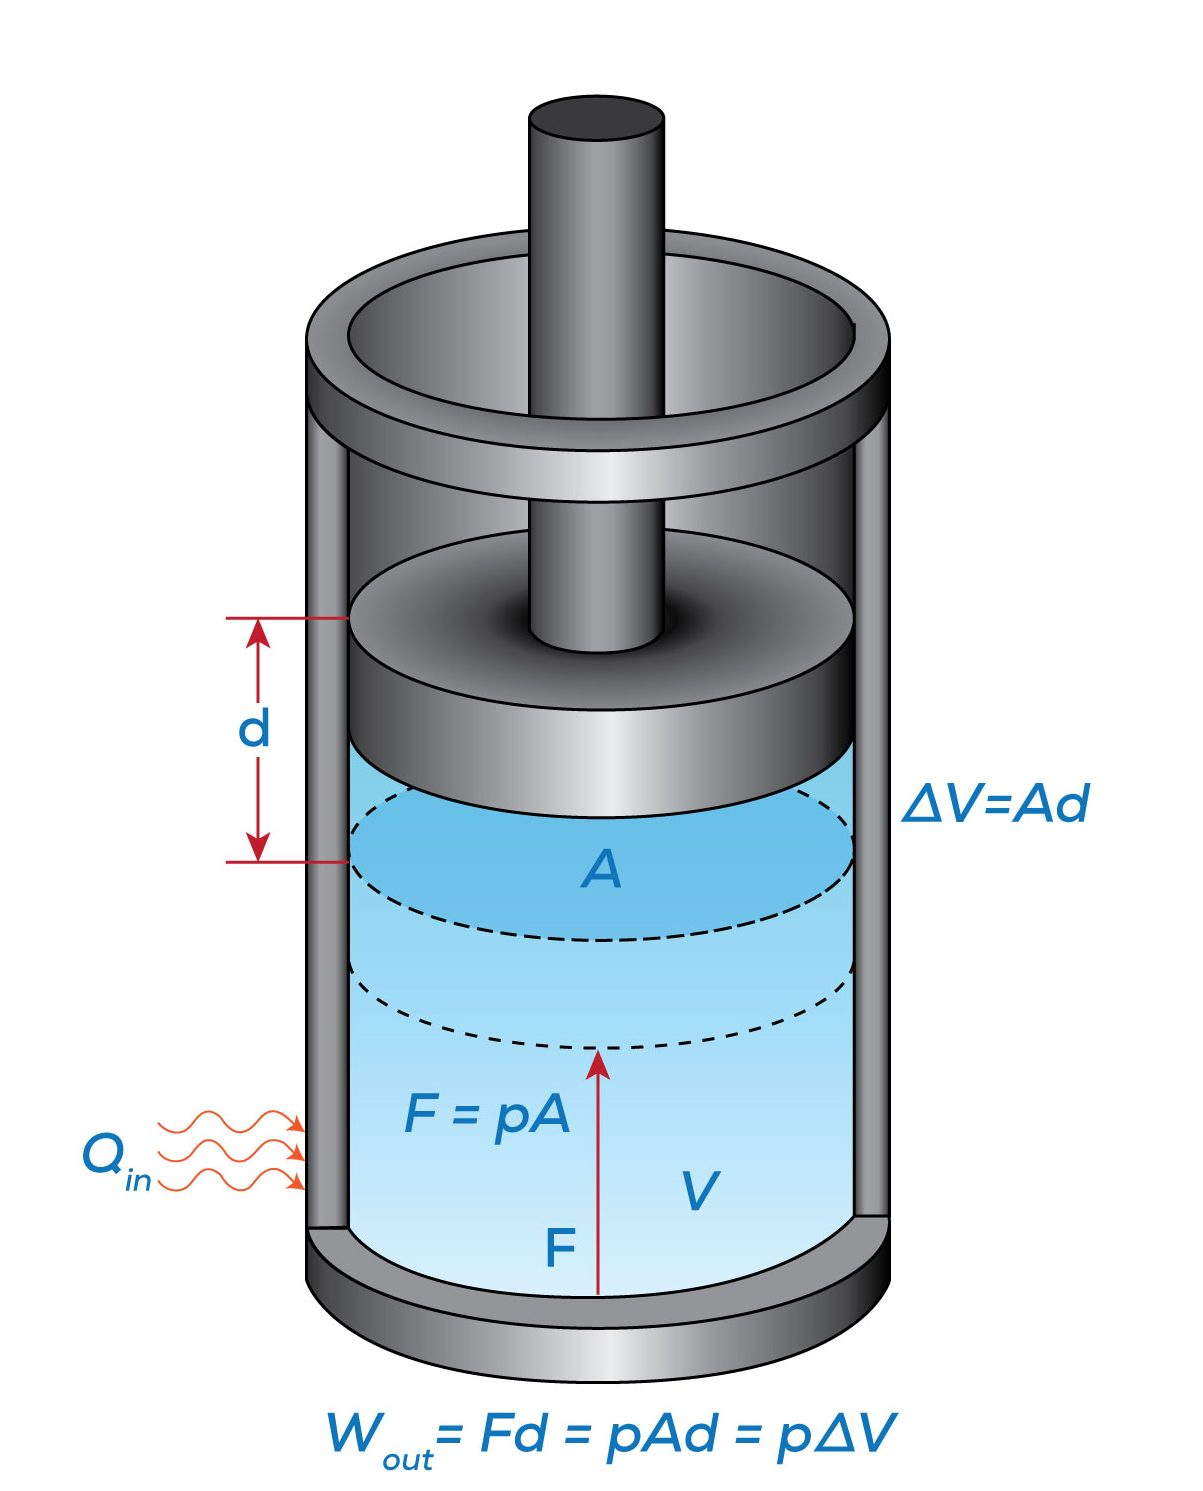
\includegraphics[width=0.3\textwidth]{Foto's-Figuren/Fig.-4-4_boundary-work1-e1626459353689.jpg}
    \caption{Arbeid verricht door een gas tijdens compressie. De kracht \(F\) werkt op de zuiger, waardoor deze zich verplaatst met een afstand \(dx\). De arbeid \(dW\) wordt gegeven door \(dW = F \cdot dx\). \footnotesize \copyright{Kh1604 is licensed under a CC BY-SA (Attribution ShareAlike) license}}
    \label{fig:work-gas-compression}
\end{figure}

\[
dW = F \cdot dx = -PAdx = -PdV
\]

Een negatief teken betekent dat een volumevergroting gepaard gaat met een negatieve arbeid, terwijl een volumeverkleining gepaard gaat met een positieve arbeid. 

Voor een quasistatisch proces geldt:
\begin{equation}
    \label{eq:hydrostatische-arbeid-algemeen}
    W = - \int_{V_i}^{V_f} PdV
\end{equation}

\begin{figure}[ht]
    \centering
    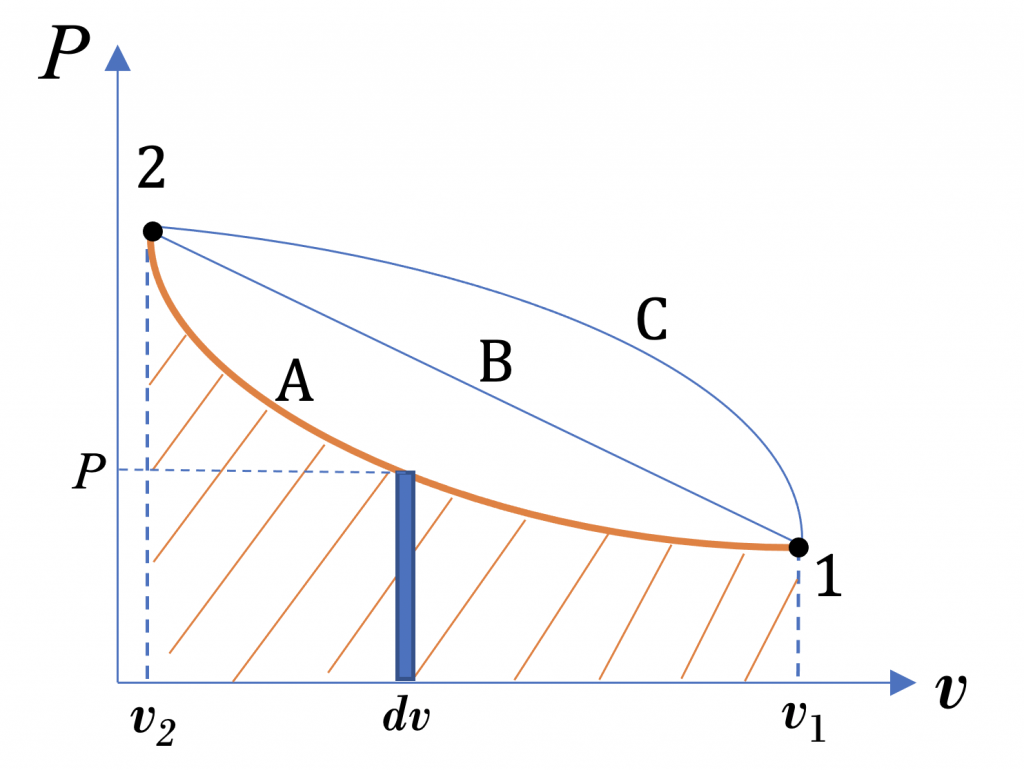
\includegraphics[width=0.3\textwidth]{Foto's-Figuren/P-v-for-boundary-work-1024x770.png}
    \caption{PV-diagram van een gas. De arbeid verricht door het gas tijdens een proces wordt gegeven door de oppervlakte onder de curve in het PV-diagram. \footnotesize \copyright{ Kh1604 is licensed under a CC BY-SA (Attribution ShareAlike) license}}
    \label{fig:work-gas-pv}
\end{figure}

Voor een quasistatisch proces is de arbeid gelijk aan de oppervlakte onder de curve in het PV-diagram. Stel we gaan van punt i naar punt f met een volume compressie:
\[
W_{if} = - \int_{V_i}^{V_f} PdV
\]
Als we van dat punt terug gaan van punt f naar punt i (en dus eeen volume expansie hebben), dan is de arbeid:
\[
W_{fi} = - \int_{V_f}^{V_i} PdV
\]
Dit betekend dat we een cyclus kunnen maken waarbij geldt \(W_{if} = -W_{fi}\). Dit is voor een quasistatisch proces langs heetzelfde pad!

Onze conventie voor cyclussen is als volgt: wijzerzin betekend dat er negatieve arbeid wordt verricht, terwijl tegenwijzerzin betekend dat er positieve arbeid wordt verricht op het systeem. Typisch zijn koelmachines tegenwijzerzin, terwijl warmtemachines wijzerzin zijn.

\subsection{Padafhankelijke Arbeid}

\begin{derivation}
    \textbf{Arbeid is padafhankelijk}: Stel we kunnen van punt 1 naar punt 2 gaan via twee verschillende paden, namelijk pad A en pad C. (Zie figuur \ref{fig:work-gas-pv}.)
    We kunnen ook een cyclus maken door van punt 1 naar punt 2 te gaan via pad C, en vervolgens terug te gaan van punt 2 naar punt 1 via pad A. De netto arbeid verricht tijdens deze cyclus is:
    \begin{align*}
        W_{cyclus} &= W_{21}(C) + W_{12}(A) 
        = -|W_{21}(C)| + |W_{12}(A)| < 0 
        \implies |W_{21}(C)| > |W_{12}(A)| \\
    \end{align*}
    Als we nu proces A van 2 naar 1 laten verlopen, dan is de netto arbeid:
    \begin{align*}
        W_{21}(A) &= -W_{12}(A) <0 \implies |W_{21}(A)| = |W_{12}(A)| \\ 
    \end{align*}
    Uit \(|W_{21}(C)| > |W_{12}(A)|\) en \(|W_{21}(A)| = |W_{12}(A)|\) volgt dat \(|W_{21}(C)| > |W_{21}(A)|\). (Of stel dat beide negatief zijn, dan is \(W_{21}(C) < W_{21}(A)\).)
    Dit betekent dat de arbeid die wordt verricht tijdens het proces van 2 naar 1 via pad C groter is dan de arbeid die wordt verricht tijdens het proces van 2 naar 1 via pad A.
    \qed
\end{derivation}
\medskip
\begin{postulate}
    \textbf{Arbeid is padafhankelijk!}
\end{postulate}

Stel we hebben een  \textbf{isobaar} proces, dan wordt de arbeid:
\begin{equation}
\label{eq:isobare-arbeid}
W = -P \int_{V_i}^{V_f} dV = -P(V_f - V_i) \qquad (P = cst)
\end{equation}
Voor een  \textbf{isochoor} proces is de arbeid triviaal 0.

\textbf{Isotherme arbeid} is dan weer een ander verhaal:
\[
W = - \int_{V_i}^{V_f} P(V)dV
\]
Waarbij de toestandsfunctie \(P(V, T)\) nu enkel van het volume afhangt \(P(V)\). 
Voor een ideaal gas is \(P = \frac{nRT}{V}\), dus de arbeid wordt:
\begin{equation}
\label{eq: isotherme-arbeid-ideaal-gas}
W = - \int_{V_i}^{V_f} \frac{nRT}{V}dV = -nRT \ln\left( \frac{V_f}{V_i} \right) \qquad (T = cst)
\end{equation} 

\textbf{Isotherme toename van druk op een vaste stof}:
\[
dV = \left( \frac{\partial V}{\partial P} \right)_T dP = - \kappa V dP \qquad (T = cst)
\]
Waar we formule \eqref{eq:isothermische-drukbaarheid} hebben gebruikt, nu volgt dat de arbeid:
\begin{equation}
\label{eq: isotherme-arbeid-vast-stof}
W = - \int_{P_i}^{P_f} \kappa VP  dP \qquad (T = cst)
\end{equation} 

Het is niet moeilijk te realiseren dat als de temperatuur constant is, een vaste stof niet veel zal uitzetten, waardoor we \(V,\kappa \approx cst\) kunnen beschouwen.

\[
W \approx \frac{\kappa V}{2} (P_f^2 - P_i^2) = \frac{\kappa m}{2\rho} (P_f^2 - P_i^2) \qquad (T = cst)
\]
Waar we gebruik hebben gemaakt van \(V = \frac{m}{\rho}\) met \(m\) de massa en \(\rho\) de dichtheid van de vaste stof.

\subsubsection{De gespannen snaar herzien}

\(\dbar W = FdL  \implies W = \int_{L_i}^{L_f} F dL\)

Herinner de wet van hooke, \(F = k(L - L_0)\), waarbij \(k\) de veerconstante is en \(L_0\) de natuurlijke lengte van de veer. De arbeid wordt:
\[W = \int_{L_i}^{L_f} k(L - L_0) dL = \frac{k}{2} \left( (L_f - L_0)^2 - (L_i - L_0)^2 \right)\]

\subsubsection{Oppervlaktefilm herzien}

\( \dbar W = Fdx = 2 \gamma ldx \). De oppervlakte van de film is \(A = 2lx\) (langs 2 kanten), dus \(dA = 2ldx\). De arbeid wordt:

\[\dbar W = \gamma dA \implies W = \int_{A_i}^{A_f} \gamma dA\]

\subsubsection{Elektrolyse cel herzien}

\( \dbar W = V_\epsilon dQ \) met \(dQ\) het aantal verplaatste elektronen inde cel tijdens de reactie en \(V_\epsilon\) de elektrische potentiaal. De arbeid wordt: 
\[W = \int_{Q_i}^{Q_f} V_\epsilon dQ = \int_{t_i}^{t_f} V_\epsilon \frac{dQ}{dt} dt = \int_{t_i}^{t_f} V_\epsilon I dt\]

\subsubsection{Verandering vd polarisatie van een diëlektricum herzien}

\begin{figure}[ht]
    \centering
    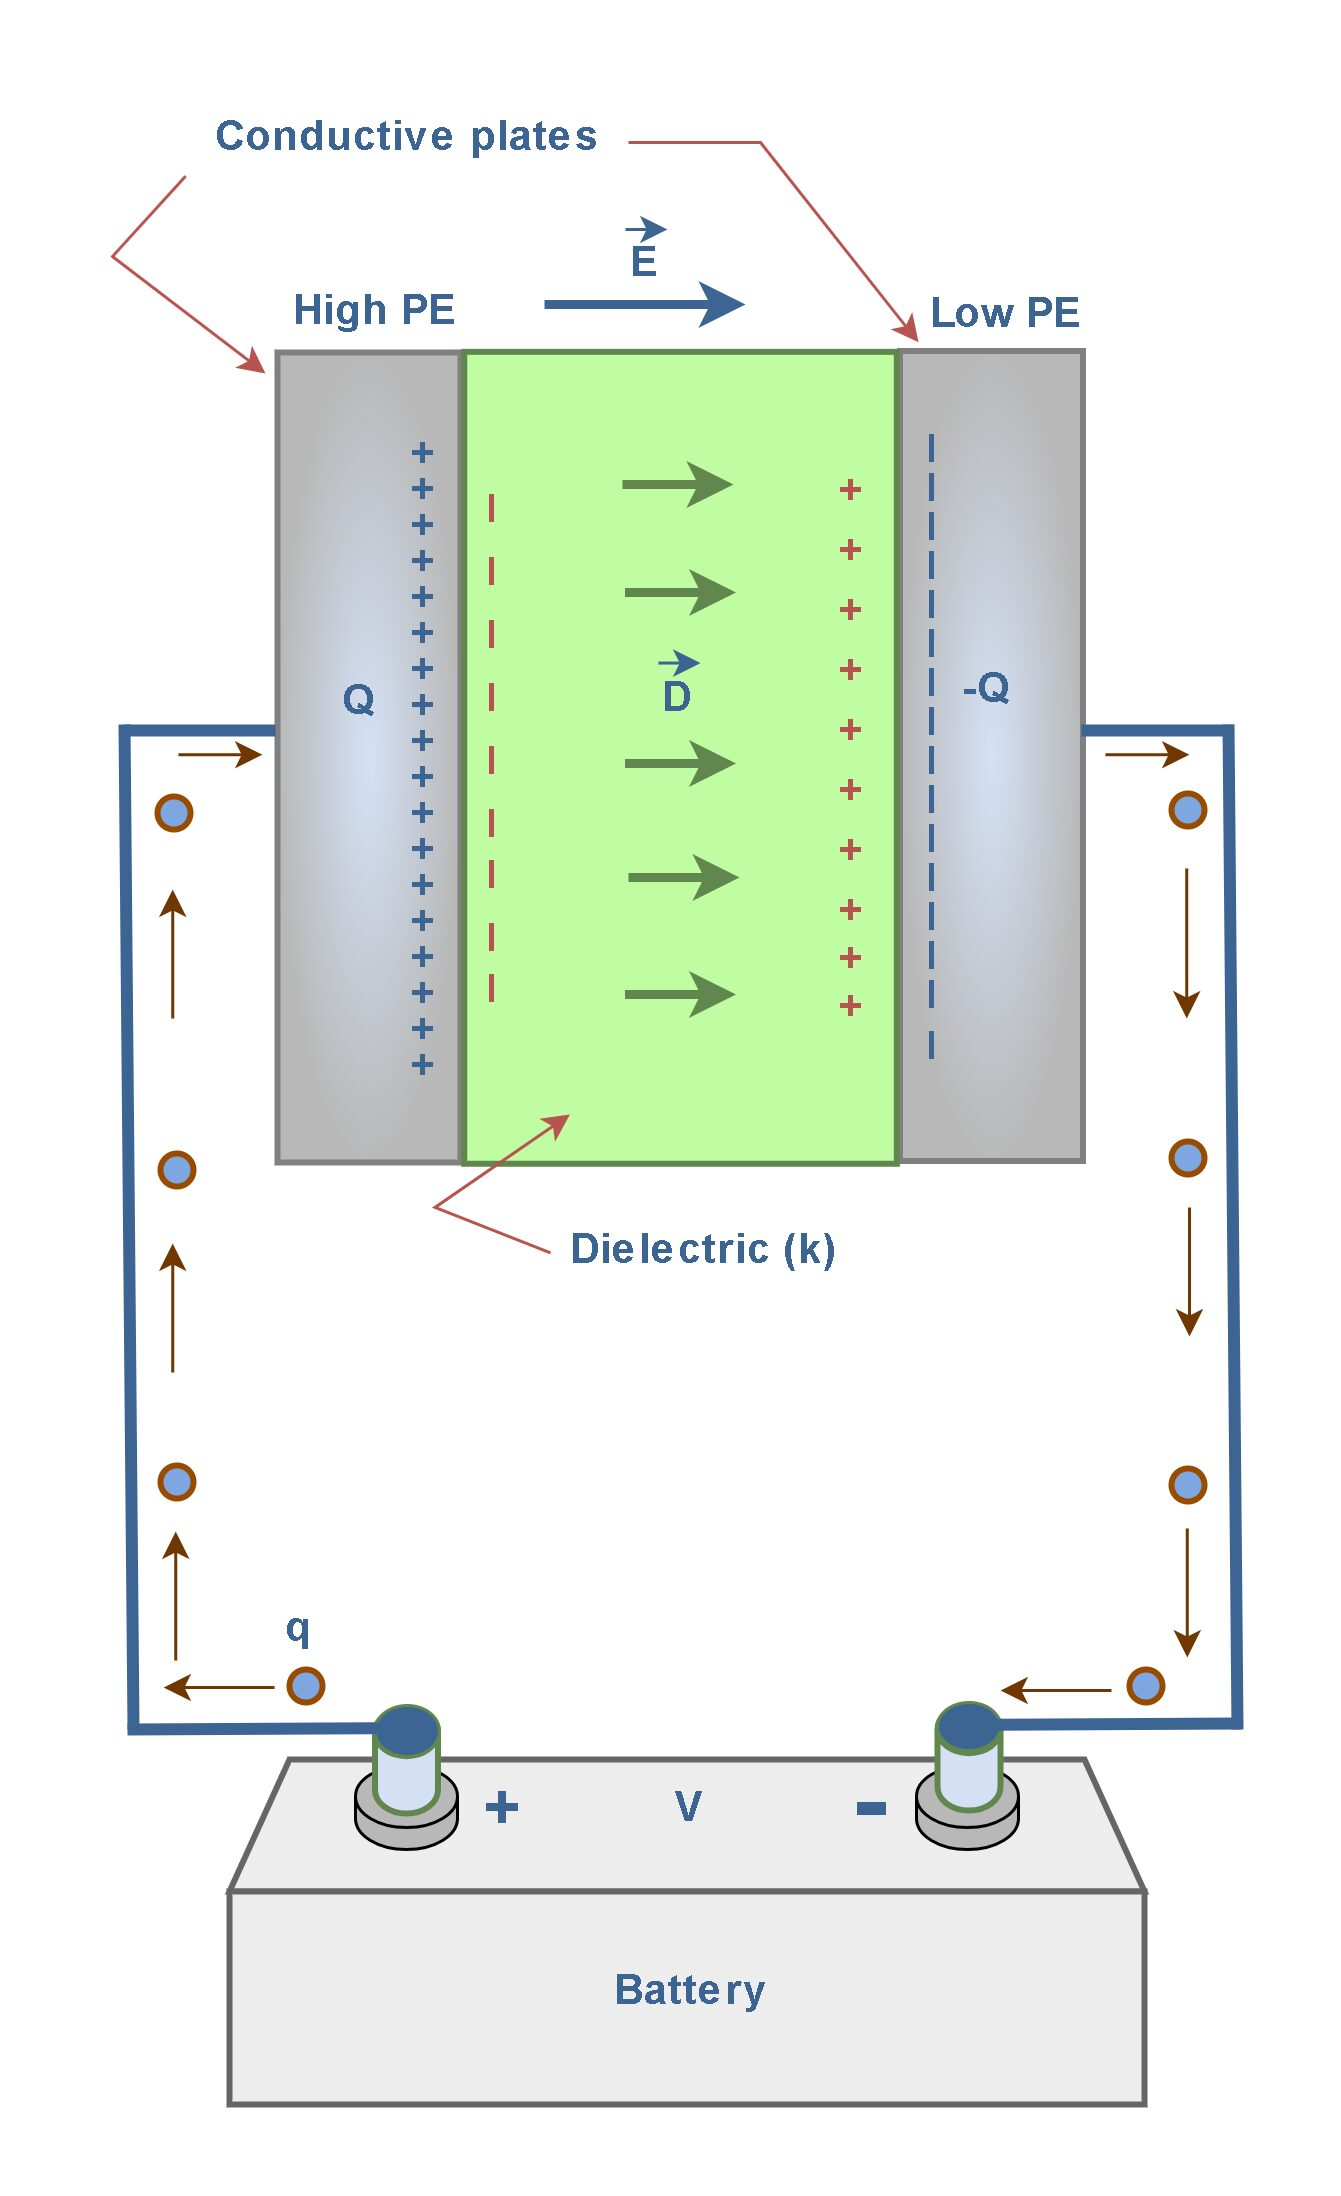
\includegraphics[width=0.5\textwidth]{Foto's-Figuren/Electric-Displacement.jpeg}
    \caption{Een diëlektricum tussen twee platen van een condensator. Wanneer er een elektrisch veld wordt aangelegd, worden de moleculen in het diëlektricum gepolariseerd, wat resulteert in een verandering van de polarisatie \(\Pi\) van het diëlektricum.
        \footnotesize \copyright{ September 29, 2024 by Kamran Jalilinia site: \url{https://www.electronics-lab.com/article/electric-displacement-and-electrostatic-energy/}}}
    \label{fig:di-electric-polarization}
\end{figure}


\(\dbar W = V_\epsilon dQ =EldQ\) met \(E = \frac{V_\epsilon}{l}\) het elektrische veld. (zie figuur \ref{fig:di-electric-polarization}) 

\(Q = A(\bm D \cdot \bm n) \) met \(\bm n\) de normaal op het oppervlak (in ons geval staat alles loodrecht dus wordt dit geen probleem).

\(\dbar W = ElAdD = EVdD \) met \(V\) nu het volume vh dielektricum (wordt constant beschouwd).

Uit \(\bm D = \epsilon_0 \bm E + \frac{\bm \Pi}{V} \implies dD = \epsilon_0 dE + \frac{d\Pi}{V}\) (\(V\) = cst) volgt:

\[\dbar W = EVdD = \epsilon_0 E dE V + E d\Pi\]

Doordat enkel de tweeede term de polarisatie beïnvloed negeren we de eerste term, en krijgen we:
\[\dbar W = E d\Pi \implies W = \int_{\Pi_i}^{\Pi_f} E d\Pi\]



\subsubsection{Verandering vd magnetisatie van een magnetisch materiaal herzien}

\begin{figure}[ht]
    \centering
    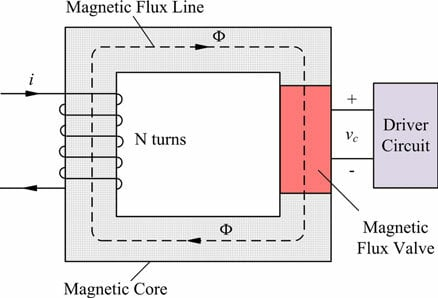
\includegraphics[width=0.5\textwidth]{Foto's-Figuren/arbeid-magnetisatie.jpeg}
    \caption{Een spoel met N windingen (magneetventiel). \footnotesize \copyright{ Magnetic Flux Valve: A Magnetoelectric Materials-Based Device for Conversion and Control of Electric Power - Scientific Figure on ResearchGate. Available from: \url{https://www.researchgate.net/figure/Simple-magnetic-circuit-containing-an-MFV_fig1_305802042} [accessed 10 May 2026] }}
    \label{fig:magnetization-work}
\end{figure}

Uit de inductiewet van Faraday volgt dat \( V_\epsilon = \frac{d\Phi}{dt} = -NA \frac{dB}{dt} \) met (\(A = cst\) en \(N\) het aantal windingen van de spoel zie figuur \ref{fig:magnetization-work}). 

\[\dbar W = -V_\epsilon dQ = -NA \frac{dB}{dt} dQ = -NA \frac{dQ}{dt} dB = -NAI dB \]

De magnetische veldsterkte \(H\) is gedefinieerd als \(H = \frac{NI}{l}\), dus \(NI = Hl \implies NIA = HV\).

\[\implies \dbar W = -HV dB\]

We moeten nog rekening houden met de differentiaal van \(B\). Herinner \(B = \mu_0(H + \frac{M}{V})\), dus \(dB = \mu_0(dH + \frac{dM}{V})\).

Dus \[\dbar W = -HV \mu_0(dH + \frac{dM}{V}) = -HV \mu_0 dH - H\mu_0 dM\]
We kunnen de eerste term negeren, omdat deze niet bijdraagt aan de verandering van de magnetisatie:

\[\dbar W = -\mu_0 H dM \implies W = -\mu_0 \int_{M_i}^{M_f} H dM\]

\subsection{Samengestelde Systemen}

Nu rest ons alleen nog te zien hoe we de arbeid kunnen berekenen voor samengestelde systemen, waarbij meerdere processen tegelijkertijd plaatsvinden.
In dit geval kunnen we de totale arbeid berekenen door de arbeid van elk proces afzonderlijk te berekenen en deze vervolgens op te tellen.
Dit is mogelijk omdat arbeid een additieve grootheid is, wat betekent dat de totale arbeid gelijk is aan de som van de arbeid van elk proces.

\begin{figure}[ht]
    \centering
    \includegraphics[width=0.5\textwidth]{Foto's-Figuren/Carnot_heat_engine_2.pdf}
    \caption{Een samengesteld systeem.  \footnotesize \copyright{Wikipedia contributor}}
    \label{fig:composite-system}
\end{figure}

Zo een samengesteld systeem kan vanalles zijn. Als we eens kijken naar 2 hydrostatische systemen A en B geïsolleerd met elkaar. Maar ze staan onrechtsreeks in contact met elkaar via een diathermischee wand met een reservoir C, dan hebben we 5 coordinaten: \(P_A, V_A, P_B, V_B\) en \(T_C =T\).

Er zijn 2 toestandsfuncties \( f_A(P_A,V_A, T) = 0\) en \(f_B(P_B,V_B, T) = 0\). De arbeid kan berekend worden aan de hand van:

\[\dbar W = -P_AdV_A - P_BdV_B\]

Dit kunnen we ook doen voor gelijk welke combinties van de voorgaande processen, zolang we maar de juiste toestandsfuncties en de bijbehorende differentiaalvergelijkingen hebben.

Algemeen geldt:
\[\dbar W = \sum_i Y_i dX_i\]
waarbij \(Y_i\) de veralgemeende kracht is die werkt op de veralgemeende verplaatsing \(X_i\). In het geval van ons eerdere hydrostatisch systeem is \(Y_i = -P\) en \(X_i = V\), terwijl in het geval van een gespannen snaar \(Y_i = F\) en \(X_i = L\) is, enzovoort.
\section{Warmte en Eerste Wet}
\subsection{Arbeid en Warmte}
Het is mogelijk de toestand van een systeem te veranderen zonder arbeid te verrichten. 

\begin{definition}
    \textbf{Adiabatische Arbeid}: Arbeid die wordt verricht zonder warmte-uitwisseling.
\end{definition}
\begin{definition}
    \textbf{Warmte}: Energie die wordt overgedragen tussen systemen als gevolg van een temperatuurverschil.
\end{definition}

Doordat een adiabatische wand geen warmte-uitwisseling toelaat, wordt deze een warmte-isolator genoemd. Een diathermische wand is een warmtegeleider.

\subsection{Inwendige Energie}

\begin{postulate}
    \textbf{Eerste Wet van de Thermodynamica}: De verandering in inwendige energie van een systeem is gelijk aan de som van de warmte die aan het systeem wordt toegevoegd en de arbeid die aan het systeem wordt verricht.
    \begin{equation}
        \Delta U = Q + W
    \end{equation}
    Waarbij:
    \begin{itemize}
        \item $\Delta U$ de verandering in inwendige energie is,
        \item $Q$ de warmte is die aan het systeem wordt toegevoegd (positief als het systeem warmte ontvangt, negatief als het warmte afgeeft),
        \item $W$ de arbeid is die aan het systeem wordt verricht (positief als er arbeid op het systeem wordt verricht, negatief als het systeem arbeid verricht).
    \end{itemize}   
\end{postulate}

\begin{definition}
    \textbf{Inwendige Energie functie}: De inwendige energie $U$ is een functie van de toestand van het systeem, en kan worden uitgedrukt als $U = U(S, V, N)$, waarbij $S$ de entropie is, $V$ het volume, en $N$ het aantal deeltjes.
    (Zie H9)
\end{definition}


\subsection{Wiskunde van de Eerste Wet}

De wiskundige formuleringg van de eerste wet hierboven bevat drie belanrijke ideëen:
\begin{itemize}
    \item De verandering in inwendige energie $\Delta U$ is een functie van de toestand van het systeem, en is dus een toestandsgrootheid. Het hangt alleen af van de begin- en eindtoestand van het systeem.
    \item Behoud energie
    \item Definitie van warmte als energieoverdracht als gevolg van een temperatuurverschil.
\end{itemize}
   

Een infinitesimaale hoeveelheid warmte \(\dbar Q\) kan niet worden uitgedrukt als differentiaal en is geen toestandsfunctie!

\begin{derivation}
    \textbf{Dubbelsysteem met adiabatische wand} dan geldt:
    \[ \Delta U_A = Q_A + W_A \] 
    en
    \[ \Delta U_B = Q_B + W_B \]
    \begin{align*}
        \implies \
        \Delta U_A + \Delta U_B &= (Q_A + Q_B) + (W_A + W_B)
    \end{align*}
        Omdat de wand adiabatisch is, is er geen warmte-uitwisseling tussen de systemen, dus \(Q_A + Q_B = 0\). Daarom kunnen we de vergelijking vereenvoudigen tot:
    \begin{align*}
        \Delta U_A + \Delta U_B &= W_A + W_B
    \end{align*}
    In adiabatische omstandigheden is de warmte verloren of gewonnen door het ene systeem gelijk aan de warmte gewonnen of verloren door het andere systeem.
    \qed
\end{derivation}


\subsection{Eerste Wet in Differentiaalvorm}

Voor een infinitesimale verandering in de toestand van het systeem kunnen we de eerste wet van de thermodynamica schrijven als:
\begin{equation}
    dU = \dbar Q + \dbar W
\end{equation}
Waarbij \(dU\) de differentiaal van de inwendige energie is, \(\dbar Q\) de infinitesimale hoeveelheid warmte is die aan het systeem wordt toegevoegd, en \(\dbar W\) de infinitesimale hoeveelheid arbeid is die aan het systeem wordt verricht.
Maar dit zou ondertussen niet meer hoeven uitgelegd te worden.

In ons hydrostatisch systeem:
\[
dU = \dbar Q - PdV
\]
In een dubbel hydrostatisch systeem:
\[
dU_A + dU_B = \dbar Q_A + \dbar Q_B - P_A dV_A - P_B dV_B
\]

De inwendige energie voor alle andere eerdere geziene systemen kunnen analoog bepaald worden:
\begin{itemize}
    \item Gespannen snaar: \(dU = \dbar Q + FdL\)
    \item Oppervlaktefilm: \(dU = \dbar Q + \gamma dA\)
    \item Elektrische cel: \(dU = \dbar Q + V_\epsilon dZ\) 
    
    (Hier gebruiken we \(Z\) voor de ladingen om dit niet te verwarren met de warmte \(Q\))
    \item Diëlektricum: \(dU = \dbar Q + E d\Pi\)
    \item Magnetisch systeem: \(dU = \dbar Q + \mu_0 H dM\)
\end{itemize}

Waarbij we analoog deze systemen kunnen combineren in een dubbel of zelf meervooudig systeem.

\begin{definition}
    \textbf{Pfaffiaanse differentiaalvormen}: De differentiaalvormen die voorkomen in de eerste wet van de thermodynamica, zoals \(dU\), \(\dbar Q\), en \(\dbar W\), worden Pfaffiaanse differentiaalvormen genoemd.
    Deze vormen zijn niet-exact, wat betekent dat ze niet kunnen worden uitgedrukt als de totale differentiaal van een functie van de toestand van het systeem.
    Als er maar twee verandelijken zijn, kan er wel steeds een integrerende factor worden gevonden, maar bij meer dan twee veranderlijken is dit niet altijd mogelijk. 
    Die integrerende factor zorgt ervoor dat de uitdrukking een totale differentiaal wordt, en dus een toestandsfunctie kan worden gedefinieerd.
\end{definition}


\subsection{Warmtecapaciteit}

\begin{definition}
    \textbf{Gemiddeldee Warmtecapaciteit}: 
    \[\bar{C} = \frac{Q}{T_f-T_i}\]
    Als Q en T infinitesimaal klein worden, kunnen we de gemiddelde warmtecapaciteit benaderen door de differentiaalvorm:
    \[C = \lim_{T_F \to T_i} \frac{Q}{T_f - T_i} =\frac{\dbar Q}{dT}\]
\end{definition}

\begin{definition}
    \textbf{Soortelijke Warmtecapaciteit}: De soortelijke warmtecapaciteit \(c\) is de warmtecapaciteit per eenheid massa van een stof, gedefinieerd als:
\[c = \frac{C}{m} = \frac{\dbar Q}{m dT}\]
Waarbij \(m\) de massa van de stof is.
\end{definition}

\begin{definition}
    \textbf{Molaire Warmtecapaciteit}: De molaire warmtecapaciteit \(C_m\) is de warmtecapaciteit per mol van een stof, gedefinieerd als:
\[C_m = \frac{C}{n} = \frac{1}{n}\frac{\dbar Q}{ dT}\]
Waarbij \(n\) het aantal mol van de stof is.
\end{definition}

\begin{definition}
    \textbf{Warmtecapaciteit bij constante druk}:
    \[C_P = \left( \frac{\dbar Q}{dT} \right)_P\]
\end{definition}

\begin{definition}
    \textbf{Warmtecapaciteit bij constant volume}:
    \[C_V = \left( \frac{\dbar Q}{dT} \right)_V\]
\end{definition}

We kunnen deze warmtecapaciteiten ook uitschrijven voor onze voorgaande systemen:
\begin{itemize}
    \item Hydrostatisch systeem: \(C_P = \left( \frac{\dbar Q}{dT} \right)_P\) en \(C_V = \left( \frac{\dbar Q}{dT} \right)_V\)
    \item Gespannen snaar: \(C_F = \left( \frac{\dbar Q}{dT} \right)_F\) en \(C_L = \left( \frac{\dbar Q}{dT} \right)_L\)
    \item Oppervlaktefilm: \(C_A = \left( \frac{\dbar Q}{dT} \right)_A\) en \(C_\gamma = \left( \frac{\dbar Q}{dT} \right)_\gamma\)
    \item Elektrische cel: \(C_{V_\epsilon} = \left( \frac{\dbar Q}{dT} \right)_{V_\epsilon}\) en \(C_Z = \left( \frac{\dbar Q}{dT} \right)_Z\)
    \item Diëlektricum: \(C_E = \left( \frac{\dbar Q}{dT} \right)_E\) en \(C_\Pi = \left( \frac{\dbar Q}{dT} \right)_\Pi\)
    \item Magnetisch systeem: \(C_H = \left( \frac{\dbar Q}{dT} \right)_H\) en \(C_M = \left( \frac{\dbar Q}{dT} \right)_M\)
\end{itemize}

\begin{definition}
    \textbf{Warmtereservoire}: Een warmtereservoire is een systeem met een zeer grote warmtecapaciteit, waardoor de temperatuur van het systeem bij het toevoegen of afvoeren van warmte vrijwel constant blijft.
\end{definition}

Voor een isobaar proces is de warmtecapaciteit:
\[C_P = \left( \frac{\dbar Q}{dT} \right)_P \implies Q_P = \int_{T_i}^{T_f} C_P dT = C_P (T_f - T_i)\]
Voor een isochor proces is de warmtecapaciteit:
\[C_V = \left( \frac{\dbar Q}{dT} \right)_V \implies Q_V = \int_{T_i}^{T_f} C_V dT = C_V (T_f - T_i)\]

Stel we kijken nu terug naar ons hydrostatisch systeem (\(\dbar Q = dU+PdV\)), dan kunnen we de warmtecapaciteit bij constante druk en constant volume ook uitdrukken in termen van \(U\):
\[U(T,V) \implies dU = \left( \frac{\partial U}{\partial T} \right)_V dT + \left( \frac{\partial U}{\partial V} \right)_T dV\]
\[U(P,T) \implies dU = \left( \frac{\partial U}{\partial P} \right)_T dP + \left( \frac{\partial U}{\partial T} \right)_P dT\]
\begin{align*}
    C_V &= \left( \frac{\dbar Q}{dT} \right)_V = \left( \frac{\partial U}{\partial T} \right)_V \\
    C_P &= \left( \frac{\dbar Q}{dT} \right)_P = \left( \frac{\partial U}{\partial T} \right)_P + P \left( \frac{\partial V}{\partial T} \right)_P
\end{align*}

\subsubsection{Inwendige energie van een gas}

Tijdens een \textbf{Vrije expansie} van een gas, waarbij het gas zich uitbreidt in een vacuüm zonder externe druk, is er geen arbeid verricht en geen warmte-uitwisseling (\(dU = dW = 0\)).
Dit impliceert dat de temperatuur oook niet verandert (\(dT = 0\)).

Gevolgen:
\[\left( \frac{\partial U}{\partial V} \right)_T = 0\]
\(U\) is volume onafhankelijk.
\[\left( \frac{\partial U}{\partial P} \right)_T = 0\]
Analoog is \(U\) druk onafhankelijk.

\subsubsection{Geval Ideaal Gas}

Voor eeen ideaal gas geldt:
\[PV = nRT\]
\textbf{Per definitie van een ideaal gas} geldt ook:
\[\left( \frac{\partial U}{\partial P} \right)_T = 0\]
Dit kan worden aangetoont in Hoofdstuk 9 door de iideale gaswet in de tweede energievergelijking te substitueren.

We kunnen:
\[\left( \frac{\partial U}{\partial P} \right)_T = \left( \frac{\partial U}{\partial V} \right)_T \left( \frac{\partial V}{\partial P} \right)_T  = 0\]
Met:
\[\left( \frac{\partial V}{\partial P} \right)_T = nRT\left( \frac{\partial \frac{1}{P}}{\partial P} \right)_T =-\frac{nRT}{P^2}\]
Ook herschrijven als:
\[\left( \frac{\partial U}{\partial P} \right)_T = -\frac{nRT}{P^2} \left( \frac{\partial U}{\partial V} \right)_T = 0 \implies \left(\frac{\partial U}{\partial V}\right)_T = 0\]

Hieruit leiden we af dat \(U = U(T)\) een functie is van de temperatuur alleen, en niet van het volume of de druk. Dit is een kenmerk van ideale gassen!

Uit \(C_V = \frac{dU}{dT}\) wordt de eerste hoofdwet voor een ideaal gas:
\begin{equation}
    \label{eq:1e-HW-C_V}
    \dbar Q = C_V dT + PdV
\end{equation}

De differentiatie van de ideale gaswet \(PV = nRT\) geeft:
\[PdV + VdP = nRdT\]
Hieruit kunnen we \(PdV\) vervangen in de eerste hoofdwet:
\[\dbar Q = C_V dT + nRdT - VdP = (C_V + nR) dT - VdP\]
\[\implies \frac{\dbar Q}{dT} = (C_V + nR) - V \left( \frac{dP}{dT} \right)\]
Hieruit kunnen we de warmtecapaciteit bij constante druk bepalen:
\[C_P  = \left( \frac{\dbar Q}{dT} \right)_P = C_V + nR \qquad  (P = cst)\]

Dit verteld ons twee beelangrijke zaken:
\begin{itemize}
    \item De warmtecapaciteit bij constante druk is altijd groter dan de warmtecapaciteit bij constant volume voor een ideaal gas \footnote{Omdat er bij constante druk ook arbeid wordt verricht door het gas tijdens de expansie}.
    \item De warmtecapaciteit bij constante druk en constant volume zijn beide functies van de temperatuur alleen!
\end{itemize}

Als we \(C_P = C_V + nR\) substitueren in \(\dbar Q = C_P dT - VdP\), krijgen we:
\begin{equation}
    \label{eq:1eHW-C_P}
     \dbar Q = C_P dT - VdP
\end{equation}


\subsection{Adiabastich Proces Ideaal Gas}
\begin{derivation}
    
Voor een adiabatisch proces geldt dat er geen warmte-uitwisseling is (\(\dbar Q = 0\)). We kunnen dit toepassen op de eerste hoofdwet voor een ideaal gas:
\[0 = C_V dT + PdV\]
en
\[0 = C_P dT - VdP\]

\[\implies \frac{dP}{P} = -\frac{C_P}{C_V} \frac{dV}{V} = -\gamma \frac{dV}{V}\]
Waarbij \(\gamma = \frac{C_P}{C_V}\) de adiabatische index is of ook de verhouding van de warmtecapaciteiten genoemd.
Integreren geeft:
\[
\int_{P_i}^{P_f} \frac{dP}{P} = -\gamma \int_{V_i}^{V_f} \frac{dV}{V}
\]
\[\implies \ln \left( \frac{P_f}{P_i} \right) = -\gamma \ln \left( \frac{V_f}{V_i} \right)  = \ln \left( \frac{V_i}{V_f} \right)^\gamma\]
\[\implies \frac{P_f}{P_i} = \left( \frac{V_i}{V_f} \right)^\gamma\]
\[\implies P_i V_i^\gamma = P_f V_f^\gamma\]
Of direct:
\[\ln P = -\gamma \ln V + \ln cst\]
\[\implies  PV^{\gamma} = cst\]
\qed
\end{derivation}

Voor monoatomische gassen is \(\gamma = \frac{5}{3} = cst\), voor diatomische gassen is \(\gamma = \frac{7}{5}\) en varieert ze een beetje met de temperatuur, en voor polyatomische gassen varieert \(\gamma\) 

Merk op dat in het geval van vrije epansie een adiabatisch proces niet quasistatisch verloopt.

We kunnen ook makkelijk met de ideale gaswet volgende relaties vinden:
\[ PV^\gamma = \frac{nRT}{V} V^\gamma = nRTV^{\gamma-1} = cst \]
In het adiabatisch proces stellen we dat het aantal deeltjes \(n\) constant is:
\[TV^{\gamma -1} = cst\]
Hieruit vinden we dan nog eens:
\[TV^{\gamma -1} = T \left( \frac{nRT}{V}\right)^{\gamma-1} = T^{\gamma}(nR)^{1-\gamma} V^{1-\gamma} = cst\]
Opnieuw is \(n = cst\) en \(R = cst\):
\[\implies T^{\gamma}V^{\gamma -1} = cst\]
\[\implies TP^{\frac{1-\gamma}{\gamma}} = cst\]
De Arbeid vericht in deze quasistische expansie van een ideaal gas wordt:
\begin{align*}
    W &= -\int_{V_i}^{V_f} PdV = -\int_{V_i}^{V_f} \frac{cst}{V^\gamma} dV = -cst \int_{V_i}^{V_f} V^{-\gamma} dV \\
    &= -\frac{cst}{1-\gamma} \left( V_f^{1-\gamma} - V_i^{1-\gamma} \right) = \frac{cst}{\gamma - 1} \left( V_f^{1-\gamma} - V_i^{1-\gamma} \right)
\end{align*}

Nu maken we gebruik van \(P_i V_i^\gamma = P_f V_f^\gamma = cst \):
\begin{align*}
    W &= \frac{1}{\gamma - 1} \left( P_f V_f^\gamma V_f^{1-\gamma} - P_i V_i^\gamma V_i^{1-\gamma} \right)\\
    &= \frac{1}{\gamma - 1} (P_f V_f - P_i V_i)
\end{align*}

Als de begin en eindtemperatuur bekend zijn, kunnen we dit sneller berekenen met \(PdV = -C_V dT\):
\begin{align*}
    W &= -\int_{V_i}^{V_f} PdV = \int_{T_i}^{T_f} C_V dT = C_V (T_f - T_i)
\end{align*}

\subsection{Experimentele data}

De warmtecapaciteit van vaste stoffen worden meestal bepaald aan de hand van de weerstand van een elektrische stroom,
waarbij de warmte die aan het systeem wordt toegevoegd kan worden berekend met \(Q = IVt \implies \dbar Q = I V_ dt\).
Voor metalen lijkt dit vrij logisch.

Om \(C_V \) van gassen te bepalen wordt vaak dezelfde methode toegepast, maar vaak iin een dunne metalen cilinder.
\(C_P\) wordt vaak bepaald met een doorstroomcaloriemeter.

\begin{derivation}
    Het bepalen van \(\gamma\) met de\textbf{methode van Rüchardt}:
    \begin{figure}[ht]
        \centering
        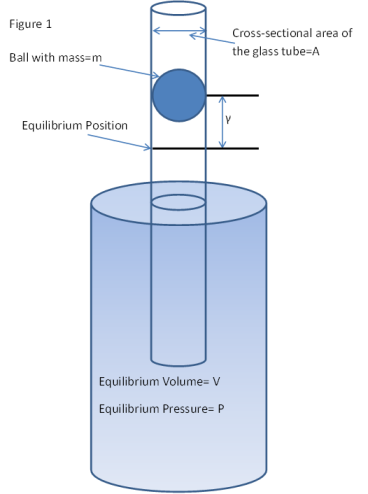
\includegraphics[width=0.5\linewidth]{Foto's-Figuren/Ruchard_experiment_layout.png}
        \caption{Schematische weergave van de methode van Rüchardt. \footnotesize \copyright{Wikipedia contributors} }
        \label{fig:Ruchard_experiment_layout}
    \end{figure}
    Een kogel met massa m wordt gebruikt als beweegbare zuiger. 
    De druk wanneer wrijving verwaarloosd wordt is:
    \[ P = P_{atm} + \frac{mg}{A} \]
    Waarbij \(A\) de oppervlakte van de kogel is. Deze oscilleert rond zijn evenwichtspositie,
    waarbij zich een klein volumeverandering plaatsvindt:
    \[\Delta V = Ay\]
    We kunnen de druk/kracht relatie \(F = A\Delta P\) gebruiken:
    \[\Delta P = \frac{F}{A}\]

    Als de kogel snel genoeg oscilleerd worden \(P\) en \(V\) als adiabatisch beschouwd een geldt \(PV^\gamma = cst\)
    of:
    \[P_\gamma V^{\gamma -1} \Delta V + V^\gamma \Delta P = 0\]
    Substitutie van \(\Delta V = Ay\) en \(\Delta P = \frac{F}{A}\) geeft:
    \[F = -\frac{\gamma PA^2 }{V}y \]

    De periode \(\tau\) wordt berekend door:
    \[\tau  = 2\pi \sqrt{\frac{m}{F}} = 2\pi \sqrt{\frac{mV}{\gamma PA^2}}\]
    Waaruit:
    \[\gamma = \frac{4\pi^2 mV}{\tau^2 PA^2}\]
    \qed
\end{derivation}

\section{Thermische Machines en de Tweede Hoofdwet}
\subsection{Van Warmte naar Arbeid}

\begin{definition}
    \textbf{Thermische Arbeidsmachines}: machines die warmte omzetten in arbeid, of omgekeerd.
\end{definition}
\begin{definition}
    \textbf{Warmtepomp}: machine die arbeid gebruikt om warmte van een koud reservoir naar een warm reservoir te transporteren.
\end{definition}

\subsection{Thermische Machines}

De eerste wet zegt ons dat \(|Q_H| - |Q_K| = |W|\).

\begin{definition}
    \textbf{Thermisch Rendement}: \(\eta = \frac{|W|}{|Q_H|} = \frac{|Q_H| - |Q_K|}{|Q_H|} = 1 - \frac{|Q_K|}{|Q_H|}\)
\end{definition}

Twee types machines:
\begin{itemize}
    \item \textbf{Uitwendige verbrandingsmachines}: machines waarbij de verbranding buiten de machine plaatsvindt, zoals stoommachines.
    \item \textbf{Inwendige verbrandingsmachines}: machines waarbij de verbranding binnen de machine plaatsvindt, zoals benzinemotoren.
\end{itemize}

\subsubsection{De Stoommachine}

\begin{definition}
    \textbf{Stoommachine}: een uitwendige verbrandingsmachine die gebruik maakt van de expansie van stoom om arbeid te verrichten.
\end{definition}    

Onze benaderende cyclus is de \textbf{Rankine-cyclus}, bestaande uit volgende zes processen:
\begin{itemize}
    \item 1\(\to\)2: Adiabatische compressie
    \item 2\(\to\)3: Isobare verwarming van water tot kookpunt.
    \item 3\(\to\)4: Isobare en isotherme verdamping.
    \item 4\(\to\)5: Isobare oververhitting van stoom.
    \item 5\(\to\)6: Adiabatische expansie van stoom.
    \item 6\(\to\)1: Isobare en isotherme condensatie van stoom.
\end{itemize}

\subsubsection{De Stirlingmotor}

De geïdealiseerde cyclus van een Stirlingmotor bestaat uit volgende vier processen:
\begin{itemize}
    \item 1\(\to\)2: Isotherme compressie van het gas bij lage temperatuur \(T_K\).
    \item 2\(\to\)3: Isochore warmteopname waarbij het gas wordt opgewarmd van \(T_K\) naar \(T_H\).
    \item 3\(\to\)4: Isotherme expansie van het gas bij hoge temperatuur \(T_H\).
    \item 4\(\to\)1: Isochore warmteafvoer waarbij het gas wordt gekoeld van \(T_H\) naar \(T_K\).
\end{itemize}

De geïdealiseerde cyclus steunt op vijf veronderstellingen:
\begin{itemize}
    \item Het werkmedium is een ideaal gas.
    \item Er zijn geen lekken.
    \item De warmte gaat niet verloren aan de omgeving door de wanden.
    \item De regenerator is een perfecte thermische isolator.
    \item Er is geen wrijving.
\end{itemize}


\subsubsection{De Benzinemotor}

Het viertaktproces van een benzinemotor bestaat uit vier bewegingen. Voor de volledigheid worden zes processen beschreven:
\begin{itemize}
    \item Inlaat (1e beweging): het inlaatventiel opent en het mengsel van lucht en brandstof wordt aangezogen.
    \item Compressie (2e beweging): het mengsel wordt samengeperst, waardoor de temperatuur en druk stijgen.
    \item Ontsteking: het mengsel wordt ontstoken, meestal door een vonk, wat leidt tot een snelle verbranding en expansie van gassen.
    \item Expansie (3e beweging): de hete gassen duwen de zuiger naar beneden, waardoor arbeid wordt verricht.
    \item Eerste uitlaat: het uitlaatventiel opent en de verbrande gassen worden afgevoerd.
    \item Tweede uitlaat (4e beweging): de zuiger beweegt omhoog om de laatste restanten van de verbrande gassen uit te duwen.
\end{itemize}

De bekendste cyclus hiervan is de \textbf{Otto-cyclus}, genaamd achter een vriend van Miel, bestaande uit volgende zes (waarvan vier essentieel) processen:
\begin{itemize}
    \item 1\(\to\)2: Quasistatische adiabatische compressie van het gas.
    \item 2\(\to\)3: Quasistatisch isochore temperatuur en druktoename waarbij het gas wordt verbrand en opgewarmd.
    \item 3\(\to\)4: Quasistatische adiabatische expansie van het gas.
    \item 4\(\to\)1: Quasistatisch isochore temperatuur en drukafname waarbij de verbrande gassen worden afgevoerd.
    \item 5\(\to\)1: Quasistatische isobare inlaat van het lucht-brandstofmengsel.
    \item 1 \(\to\)5: Quasistatische isobare uitlaat van de verbrande gassen bij atmosferische druk.
\end{itemize}

Hier zijn we opnieuw uitgegaan van een aantal veronderstellingen:
\begin{itemize}
    \item Het werkmedium is een ideaal gas.
    \item Alle processen zijn quasistatisch.
    \item Er is geen wrijving.
\end{itemize}

Processen 1 \(\to\) 5 en 5 \(\to \) 1 compenseren elkaar en wordt niet meer in rekening gebracht bij de berekening van het rendement.
Er zijn namelijk nog twee processen waar er warmte wordt uitgewisseld, namelijk 2 \(\to\) 3 en 4 \(\to\) 1. 
We kunnen schrijven:
\[Q_H = C_V (T_3-T_2) = |Q_H|\]
en 
\[Q_K = C_V (T_1-T_4) = -|Q_K|\]
Hieruit volgt dat het rendement van de Otto-cyclus gelijk is aan: 
\[\eta = 1 - \frac{|Q_K|}{|Q_H|} = 1 - \frac{T_4-T_1}{T_3-T_2}\]

Maar we willen een uitdrukking in functie van het volume in plaats van de temperatuur, want het volume is makkelijker te beheersen.
We kunnen hiervoor gebruik maken van de adiabatische relaties van de processen 1\(\to\)2 en 3\(\to\)4:
\[T_1 V_1^{\gamma - 1} = T_2 V_2^{\gamma - 1} \quad \text{en} \quad T_4 V_1^{\gamma - 1} = T_3 V_2^{\gamma - 1}\]
Hieruit volgt dat:
\[(T_4-T_1)V_1^{\gamma - 1} = (T_3-T_2)V_2^{\gamma - 1}\]
\[\implies \frac{T_4-T_1}{T_3-T_2} = \left(\frac{V_2}{V_1}\right)^{\gamma - 1}\]
Met \(r = \frac{V_1}{V_2}\) als compressieverhouding, kunnen we het rendement van de Otto-cyclus schrijven als:
\[\eta = 1 - \frac{|Q_K|}{|Q_H|} = 1 - \left(\frac{V_2}{V_1}\right)^{\gamma - 1} = 1 - \frac{1}{r^{\gamma - 1}}\]

\subsection{De Dieselmotor}

Er zijn opnieuw zes processen waarvan er vier nodig zijn voor de cyclus waar we geïnteresseerd in zijn:
Waar we de volgende effecten genegeren: chemische reacties, warmteverlies, wrijving, niet-ideale gassen, niet-quasistatische processen, enzovoort.   

Onze cyclus is nu de \textbf{lucht-gestandardiseerde dieselcyclus}, bestaande uit volgende zes (waarvan vier essentieel) processen:
\begin{itemize}
    \item 1\(\to\)2: Quasistatische adiabatische compressie van het gas.
    \item 2\(\to\)3: Quasistatisch isobare temperatuur en volume toename waarbij het gas wordt verbrand en opgewarmd.
    \item 3\(\to\)4: Quasistatische adiabatische expansie van het gas.
    \item 4\(\to\)1: Quasistatisch isochore temperatuur en drukafname waarbij de verbrande gassen worden afgevoerd.
    \item 5\(\to\)1: Quasistatische isobare inlaat van lucht.
    \item 1 \(\to\)5: Quasistatische isobare uitlaat van de verbrande gassen bij atmosferische druk.
\end{itemize}

Het grote verschil met de Otto-cyclus is dat het verbrandingsproces (2\(\to\)3) nu isobaar is in plaats van isochore. In deze stap zal 
\[Q_H = C_P(T_3 -T_2) = |Q_H|\]
waardoor het rendement van de dieselcyclus gelijk is aan:
\[\eta = 1 - \frac{|Q_K|}{|Q_H|} = 1 - \frac{C_V(T_4-T_1)}{C_P(T_3 - T_2)} = 1 - \frac{T_4-T_1}{\gamma (T_3 - T_2)}\]
We kunnen ook hier een uitdrukking in functie van het volume bekomen door gebruik te maken van de adiabatische relaties van de processen 1\(\to\)2 en 3\(\to\)4:
\[T_1 V_1^{\gamma - 1} = T_2 V_2^{\gamma - 1} \quad \text{en} \quad T_4 V_1^{\gamma - 1} = T_3 V_3^{\gamma - 1}\]
Hieruit volgt dat:
\[(T_4-T_1)V_1^{\gamma - 1} = T_3V_3^{\gamma - 1}-T_2V_2^{\gamma - 1}\]
\[\implies T_4-T_1 = \frac{T_3V_3^{\gamma - 1}-T_2V_2^{\gamma - 1}}{V_1^{\gamma - 1}}\]
Omdat we een isobaar hebben van 2\(\to\)3, kunnen we schrijven dat \(T_3/T_2 = V_3/V_2 \implies T_2 = T_3 \frac{V_2}{V_3}\). Hieruit volgt dat:
\[\eta = 1 - \frac{\frac{V_3^{\gamma-1}}{V_1^{\gamma-1} }- \frac{V_2^{\gamma-1}}{V_3V_1^{\gamma-1}}}{1 - \frac{V_2}{V_3}} 
= 1 - \frac{\left(\frac{V_3}{V_1}\right)^\gamma-\left(\frac{V_2}{V_1}\right)^{\gamma}}{\frac{V_3}{V_1}- \frac{V_2}{V_1}}\]
Als we de \textbf{expansieverhouding}:
\[r_E = \frac{V_1}{V_3} \]
en de \textbf{compressieverhouding}:
\[r_C = \frac{V_1}{V_2}\]
definiëren, kunnen we het rendement van de dieselcyclus schrijven als:
\[
\eta = 1 - \frac{1}{\gamma} \frac{(\frac{1}{r_E})^{\gamma} - (\frac{1}{r_C})^{\gamma}}{\frac{1}{r_E} - \frac{1}{r_C}} 
= 1 - \frac{1}{\gamma} \frac{r_E^{-\gamma} - r_C^{-\gamma}}{r_E^{-1} - r_C^{-1}}
\]

\subsection{Tweede Wet: Kelvin-Planck Formulering}

\begin{definition}
    \textbf{warme bron}: een systeem dat in staat is om warmte af te geven zonder zelf van toestand te veranderen.
\end{definition}
\begin{definition}
    \textbf{koude bron}: een systeem dat in staat is om warmte op te nemen zonder zelf van toestand te veranderen.
\end{definition}
\begin{postulate}
    Het is onmogelijk om een cyclus te hebben waarvan het enige resultaat is dat er warmte wordt onttrokken aan een warme bron en volledig wordt omgezet in arbeid. 
\end{postulate}
\begin{postulate}
    \textbf{Kelvin formulering}: "Het is onmogelijk door tussenkomst van niet-levende materie, mechanische effecten te bekomen uit een deel van deze materie, door ze af te koelen beneden de temperatuur van het koudste object in de omgeving."
\end{postulate}
\begin{postulate}
    \textbf{Planck formulering}: "Het is onmogelijk een cyclus te construeren waarvan het enige resultaat is dat er warmte wordt onttrokken aan een warme bron (warmtereservoir) en volledig wordt omgezet in arbeid."
\end{postulate}

\begin{postulate}
    \textbf{Tweede hoofdwet van de thermodynamica}: Er is geen enkel proces mogelijk waarvan het enige resultaat is dat er warmte wordt onttrokken aan een warme bron en volledig wordt omgezet in arbeid.
\end{postulate}

Een machine die de eerste hoofdwet overtreedt is een \textbf{perpetuum mobile van de eerste soort}. Een machine die de tweede hoofdwet overtreedt is een \textbf{perpetuum mobile van de tweede soort}.

\subsection{Warmtepompen}

\begin{definition}
    \textbf{Prestatiecoëfficiënt}: \(\omega= \frac{|Q_K|}{|W|} = \frac{|Q_K|}{|Q_H| - |Q_K|} = \frac{|Q_H|}{|W|} - 1\)
\end{definition}

\subsubsection{De Stirlingwarmtepomp}

De cyclus van de Stirlingmotor is reversibel, dus kunnen we deze ook gebruiken als warmtepomp.
De vier processen zijn nu:
\begin{itemize}
    \item 1\(\to\)2: Isotherme compressie van het gas bij hoge temperatuur \(T_H\).
    \item 2\(\to\)3: Isochore warmteafvoer waarbij het gas wordt gekoeld van \(T_H\) naar \(T_K\).
    \item 3\(\to\)4: Isotherme expansie van het gas bij lage temperatuur \(T_K\).
    \item 4\(\to\)1: Isochore warmteopname waarbij het gas wordt opgewarmd van \(T_K\) naar \(T_H\).
\end{itemize}

\subsubsection{De Frigo (Koelkast)}
De meeste koelmachines steunen op het \textbf{Joule-Kelvin-smoorproces}, waar men op de eigenschap van gesatureerde vloeistoffen steunt.
Het proces van de geïdealiseerde koelmachine, dus wanneer wrijving, warmteverlies, turbulentie, enzovoort worden genegeerd, bestaat uit volgende stappen:
\begin{itemize}
    \item 1\(\to\)2: Smoorproces met druk en temperatuurafname van het vloeibare koelmiddel. (Kan hier niet met thermodynamische coördinaten beschreven worden.) 
    \item 2\(\to\)3: Isotherme en isobare verdamping waarbij een hoeveelheid warmte \(Q_K\) onttrokken wordt.
    \item 3\(\to\)4: Adiabatische compressie waarbij het gasvormige koelmiddel wordt samengeperst tot een hoge druk en temperatuur.
    \item 4\(\to\)1: Isobare afkoeling waarbij het koelmiddel condenseert en warmte \(Q_H\) afgeeft aan de omgeving.
\end{itemize}

\subsection{De formulering van  Clausius voor de Tweede Hoofdwet}

\begin{postulate}
    \textbf{Clausius formulering}: "Geen enkel proces is mogelijk waarvan het enige resultaat is dat er warmte van een koud reservoir naar een warm reservoir wordt getransporteerd."
\end{postulate} 

\subsection{Gelijkwaardigheid Kelvin-Planck (K) en Clausiusformulering (C) van de Tweede Hoofdwet}

\begin{derivation}
    \textbf{Bewijs van de gelijkwaardigheid van de Kelvin-Planck en Clausius formulering van de tweede hoofdwet.}
\begin{itemize}
    \item \textbf{K \(\implies\) C}: 
    
    Stel dat een arbeidsmachine niet voldoet aan de Kelvin-Planck formulering, dan moeten we bewijzen dat ze ook niet voldoet aan de Clausius formulering.

    Stel dat er een proces is waarbij warmte van een koud reservoir naar een warm reservoir wordt getransporteerd zonder arbeid te verrichten. 
    Er wordt dus alleen een hoeveelheid warmte \(Q_1\) onttrokken van de warme bron en een arbeid \(W\) op de omgeving verricht.

        \(|Q_1| =  |W|\) 
    
    Deze arbeid wordt nu gebruikt om een warmtepomp die een hoeveelheid warmte \(Q_2\) onttrekt van een koud reservoir en een hoeveelheid warmte afgeeft aan een warm reservoir te laten werken.
    We kunnen volgens de eerste wet schrijven dat:
    \[|Q'_H | = |Q_2| + |W| = |Q_1| + |Q_2|\]
    Er is dus een netto warmteoverdracht van \(Q_2\) van het koude reservoir naar het warme reservoir, wat in strijd is met de Clausius formulering van de tweede hoofdwet.
    
    \item \textbf{C \(\implies\) K}: 
    
    Stel dat een machine niet voldoet aan de Clausius formulering, dan moeten we bewijzen dat ze ook niet voldoet aan de Kelvin-Planck formulering.

    Stel dat er een machine is die de Kelvin-Planck formulering overtreedt, dus een machine die warmte volledig omzet in arbeid. 
    Veronderstel dat de arbeidsmachine een hoeveelheid warmte \(Q_1\) onttrekt van een warme bron en een hoeveelheid arbeid \(W\) verricht, waarbij ze een hoeveelheid warmte \(|Q_2|\) afstaat aan de koude bron.
    Dan zegt de eerste hoofdwet dat:
    \[|Q_1| = |W| + |Q_2| \implies |W| = |Q_1| - |Q_2|\]
    Het netto resultaat van deze machine is dat er een hoeveelheid warmte \(|Q_1|-|Q_2|\) onttrokken wordt van een warme bron en volledig wordt omgezet in arbeid, wat in strijd is met de Kelvin-Planck formulering van de tweede hoofdwet.
\end{itemize}
\qed
\end{derivation}
\section{Reversibiliteit en de Derde Hoofdwet}

\begin{definition}[Reversibel proces]
    Een proces is \textbf{reversibel} als het systeem en zijn omgeving na het proces weer in hun oorspronkelijke toestand kunnen worden teruggebracht zonder dat er veranderingen in de omgeving optreden.
\end{definition}
\begin{definition}[Irreversibel proces]
    Een proces is \textbf{irreversibel} als het systeem en zijn omgeving na het proces niet in hun oorspronkelijke toestand kunnen worden teruggebracht zonder dat er veranderingen in de omgeving optreden.
\end{definition}

\subsection{Uitwendige mechanische irreversibiliteit}
\begin{definition}[Dissipatieve effecten]
    \textbf{Dissipatieve effecten} zijn processen waarbij energie wordt omgezet in een vorm die niet meer bruikbaar is voor het verrichten van arbeid, zoals warmte.
    Voorbeelden hiervan zijn wrijving, viscositeit en elektrische weerstand. Men zegt dat er arbeid gedissipeerd wordt.
\end{definition}

\begin{definition}[Perpetuum mobile van de derde soort]   
    Een \textbf{perpetuum mobile van de derde soort} is een hypothetisch apparaat dat in staat is om arbeid te verrichten zonder enige energiebron, door gebruik te maken van dissipatieve effecten. 
    Doordat dit niet in strijd is met de eerste twee wetten van de thermodynamica is er een derde wet nodig.
\end{definition}

\begin{definition}[Externe thermische irreversibiliteit]
    \textbf{Externe thermische irreversibiliteit} is een proces waarbij warmte wordt overgedragen van een warmer object naar een kouder object, zonder dat er enige arbeid wordt verricht. 
    Dit proces is onomkeerbaar omdat het niet mogelijk is om de warmte weer terug te laten stromen van het koudere object naar het warmere object zonder dat er arbeid wordt verricht.
\end{definition}

\begin{definition}[Interne thermische irreversibiliteit]
    \textbf{Interne thermische irreversibiliteit} is een proces waarbij warmte wordt gegenereerd binnen een systeem als gevolg van interne dissipatieve effecten, zoals wrijving of viscositeit. 
    Dit proces is niet omkeerbaar omdat het niet mogelijk is om de gegenereerde warmte weer te verwijderen zonder dat er arbeid wordt verricht.
\end{definition}

\subsection{Voorwaarden reversibiliteit}

\begin{definition}[Reversibiliteit]
    Een proces is \textbf{reversibel} als het voldoet aan de volgende voorwaarden:
    \begin{itemize}
        \item Er zijn geen dissipatieve effecten aanwezig
        \item Het proces verloopt quasistatisch 
    \end{itemize}
\end{definition}

\subsection{Reversibele Adiabatische Oppervlakken}

\begin{postulate}[Carathéodory's postulaat]
    In de nabijheid van een evenwichtstoestand van een systeem, zijn er toestanden die niet kunnen worden bereikt door een adiabatisch proces.
\end{postulate}

Herinner u een algemeen systeem met veralgemeende kracht \(Y\) en veralgemeende verplaatsing \(X\):
\[\dbar Q = dU -YdX\]
met \(U(T_e,X)\) een functie van de empirische temperatuur \(T_e\) en de veralgemeende verplaatsing \(X\).
\[
d U = \left(\frac{\partial U}{\partial T_e}\right)_X dT_e + \left(\frac{\partial U}{\partial X}_{T_e}\right) dX 
\]
\[
dU = \dbar Q + YdX \implies \dbar Q = \left(\frac{\partial U}{\partial T_e}_{X}\right) dT_e + \left[\left(\frac{\partial U}{\partial X}_{T_e}\right)  - Y\right]dX   
\]

Als we nu kijken naar een adiabatisch proces, dan is \(\dbar Q = 0\) en dus:
\[\left(\frac{\partial U}{\partial T_e}_{X}\right) dT_e + \left[\left(\frac{\partial U}{\partial X}_{T_e}\right)  - Y\right]dX = 0\]
Een oplossing voor \(\frac{dT_e}{dX}\) is:
\[\frac{dT_e}{dX} = \frac{Y - \left(\frac{\partial U}{\partial X}_{T_e}\right)}{\left(\frac{\partial U}{\partial T_e}_{X}\right)}\]
Deze oplossing is een adiabatisch oppervlak, de oplossing door een willekeurig punt kan geschreven worden als:
\[
\sigma (T_e ,X) = cst
\]

Een veralgemeend systeem met vijf coördinaten \((T_e, X, X', Y, Y')\) wordt beschreven door:
\[
\dbar Q = dU - YdX - Y'dX'
\]
met als oplossing \(\sigma (T_e, X, X')\), waarvan we de \(\sigma\) later nog zullen definieren als de entropie.

\begin{definition}
    Een \textbf{reversibel adiabatisch oppervlak} is een oppervlak in de toestandruimte van een systeem waarop alle processen adiabatisch en reversibel zijn. 
    Op dit oppervlak kunnen geen dissipatieve effecten optreden, en het proces verloopt quasistatisch. (de ruimte is ook steeds een dimensie lager dan de volledige toestandruimte.)
\end{definition}

RA-oppervlakken kunnen elkaar nooit snijden, want als ze elkaar zouden snijden,
dan zou er een punt zijn waar twee verschillende adiabatische processen elkaar kruisen, wat in strijd is met de definitie van een adiabatisch proces.

\subsection{Integreerbaarheid van dQ}


Herinner u het algemene systeem met vijf coördinaten \((T_e, X, X', Y, Y')\)? We kunnen deze uitschrijven als totale differentiaal van \(U(\sigma, X, X')\):
\[dU = \left(\frac{\partial U}{\partial \sigma}\right)_{X, X'} d\sigma + \left(\frac{\partial U}{\partial X}\right)_{\sigma, X'} dX + \left(\frac{\partial U}{\partial X'}\right)_{\sigma, X} dX'\]
We kunnen dit vergelijken met de algemene uitdrukking van \(\dbar Q\):
\[\dbar Q = dU - YdX - Y'dX' = \left(\frac{\partial U}{\partial \sigma}\right)_{X, X'} d\sigma + \left[\left(\frac{\partial U}{\partial X}\right)_{\sigma, X'} - Y\right] dX + \left[\left(\frac{\partial U}{\partial X'}\right)_{\sigma, X} - Y'\right] dX'\]

Doordat de drie coordinaten \(T_e, X, X'\) onafhankelijk zijn, moeten de volgende voorwaarden gelden:
\[\left(\frac{\partial U}{\partial \sigma}\right)_{X, X'} \neq 0\]
\[\left(\frac{\partial U}{\partial X}\right)_{\sigma, X'} = Y\]
\[\left(\frac{\partial U}{\partial X'}\right)_{\sigma, X} = Y'\]

Zodat kunnen we \(\dbar Q\) schrijven als:
\[\dbar Q = \left(\frac{\partial U}{\partial \sigma}\right)_{X, X'} d\sigma\]
We definieren nu de functie \(\lambda(\sigma)\) als:
\[\lambda(\sigma) = \left(\frac{\partial U}{\partial \sigma}\right)_{X, X'}\]
Zodat we \(\dbar Q\) kunnen schrijven als:
\[\dbar Q = \lambda(\sigma) d\sigma\]

\begin{definition}
    De functie \(\lambda(\sigma)\) wordt de \textbf{integrerende factor} genoemd, omdat het ervoor zorgt dat \(\dbar Q\) een totaal differentiaal wordt. 
    De functie \(\sigma\) wordt de \textbf{entropie} genoemd, en is een functie van de toestand van het systeem die de mate van wanorde of onomkeerbaarheid van een proces beschrijft.
\end{definition}


\begin{derivation}
We beschouwen nu twee systemen met elk drie onafhankelijke coördinaten \((T_e, Y, X)\) en \((T_e', X_H, X_H')\). Ze zijn verondersteld op elk moment in evenwicht te zijn \(T_e = T_e'\).
Samen vormen ze een samengesteld systeem met vijf onafhankelijke coördinaten \((T_e, X_H, X_R, X_H', X_R')\) \footnote{Zoals we net hebben gezien}. 

Het eerste systeem is het hoofdsysteem met coördinaten \((T_e, X_H, X_H')\) en het tweede systeem is het referentiesysteem met coördinaten \((T_e, X_R, X_R')\).
Ze hebben beiden een oplossing van de vorm \(\sigma_H (T_e, X_H, X_H')\) en \(\sigma_R (T_e, X_R, X_R')\) respectievelijk.
We veronderstellen ook dat als de twee systemen een hoeveelheid warmte \(\dbar Q\) uitwisselen, dat \(d\sigma_H\) en \(d\sigma_R\) veranderen met:
\[\dbar Q_H = \lambda_H(\sigma_H) d\sigma_H\] en \[\dbar Q_R = \lambda_R(\sigma_R) d\sigma_R\]
Waar \(\lambda_H\) en \(\lambda_R\) de integrerende factoren zijn van de respectievelijke systemen

In het samengesteld systeem zijn de RA-oppervlakken gegeven door \(\sigma (T_e, X_H, X_H', X_R, X_R') \).

We kunnen de twee systemen  \(X_H'\) en \(X_R'\) uitdrukken in termen van \(T_e,X_H, \sigma_H\) en \(T_e, X_R, \sigma_R\) respectievelijk.
Zodat de coördinaten \(X_H'\) en \(X_R'\) kunnen worden geëlimineerd uit de vergelijking van het samengestelde systeem, en we kunnen schrijven:
\[\sigma_c = \sigma_c (T_e, X_H, X_R, \sigma_H, \sigma_R) \]
Waar \(\lambda_c\) een functie is die de relatie tussen de entropieën van de twee systemen beschrijft. 
En analoog als daarnet \( \dbar Q_c = \lambda_c(\sigma) d\sigma\) kunnen we schrijven:

We kunnen dus schrijven:
\tiny
\[d\sigma_c = \left(\frac{\partial \sigma_c}{\partial \sigma_H}\right)_{T_e, X_H, \sigma_R , X_R} d\sigma_H
 + \left(\frac{\partial \sigma_c}{\partial \sigma_R}\right)_{ T_e, X_H, \sigma_H, X_R} d\sigma_R
+ \left(\frac{\partial \sigma_c}{\partial T_e}\right)_{X_H, \sigma_H, X_R, \sigma_R} dT_e 
+ \left( \frac{\partial \sigma_c}{\partial X_H} \right)_{T_e, \sigma_H, \sigma_R, X_R} dX_H
+ \left(\frac{\partial \sigma_c}{\partial X_R} \right)_{T_e, \sigma_H, \sigma_R, X_H} dX_R\]
\normalsize

Veronderstel dat een reversibel proces de warmteoverdracht \(\dbar Q_c\) tussen het warmtereservoir en het gecombineerde systeem opsplitst in een warmteoverdracht \(\dbar Q\)
naar het hoofdsysteem en een warmteoverdracht \(\dbar Q_R\) naar het referentiesysteem, zodat:
\begin{align*}
    \dbar Q_c &= \dbar Q + \dbar Q_R\\
    \implies \lambda_c d\sigma_c &= \lambda_H d\sigma_H + \lambda_R d\sigma_R\\
    \implies d\sigma_c &= \frac{\lambda_H d\sigma_H}{\lambda_c} + \frac{\lambda_R d\sigma_R}{\lambda_c}
\end{align*}
Pluggen we dit in onze hele lange vergelijking van nu net, dan vinden we:
\begin{align*}
    \frac{\lambda_H}{\lambda_c} &= \left(\frac{\partial \sigma_c}{\partial \sigma_H}\right)_{T_e, X_H, \sigma_R , X_R}
    \implies \frac{\lambda_H}{\lambda_c} = \frac{\partial \sigma_c}{\partial \sigma_H} \\
    \frac{\lambda_R}{\lambda_c} &= \left(\frac{\partial \sigma_c}{\partial \sigma_R}\right)_{ T_e, X_H, \sigma_H, X_R}
    \implies \frac{\lambda_R}{\lambda_c} = \frac{\partial \sigma_c}{\partial \sigma_R} \\
    0 &= \left(\frac{\partial \sigma_c}{\partial T_e}\right)_{X_H, \sigma_H, X_R, \sigma_R} 
    \implies \frac{\partial \sigma_c}{\partial T_e} = 0 \\
    0 &= \left( \frac{\partial \sigma_c}{\partial X_H} \right)_{T_e, \sigma_H, \sigma_R, X_R} 
    \implies \frac{\partial \sigma_c}{\partial X_H} = 0 \\
    0 &= \left(\frac{\partial \sigma_c}{\partial X_R} \right)_{T_e, \sigma_H, \sigma_R, X_H}
    \implies \frac{\partial \sigma_c}{\partial X_R} = 0
\end{align*}

Dit zegt ons iets heel belangrijks, namelijk \(\sigma_c\) van de twee systemen gerelateerd zijn door een functie van de entropieën van de twee systemen, en dat \textbf{deze functie alleen afhankelijk is van de entropieën (nu nog \(\sigma_H\) en \(\sigma_R\)) en niet van de andere coördinaten (zoals \(T_e\), \(X_H\), en \(X_R\) zoals net aangetoond).}

Dus we kunnen \(\sigma_c\) schrijven als:
\[\sigma_c = \sigma_c(\sigma_H, \sigma_R)\]
met zoals net berekend:
\[\frac{\lambda_H}{\lambda_c} = \frac{\partial \sigma_c}{\partial \sigma_H}\] en \[\frac{\lambda_R}{\lambda_c} = \frac{\partial \sigma_c}{\partial \sigma_R}\]
Dus de deze verhoudingen zijn niet afhankelijk van de andere coördinaten, maar alleen van de entropieën van de twee systemen.

Maar waarvan zijn ze nu wel nog afhankelijk?
\begin{align*}
    \lambda_H &= \phi(T_e, X_H, X_R) f(\sigma_H) = \phi(T_e)f(\sigma_H) \\
    \lambda_R &= \phi(T_e, X_H, X_R) g(\sigma_R) = \phi(T_e)g(\sigma_R) \\
    \sigma_c &= \sigma_c(T_e, X_H, X_R) h(\sigma_H, \sigma_R) = \phi(T_e)h(\sigma_H, \sigma_R) \\ 
\end{align*}
Doordat \(\lambda_H\) niet afhankelijk is van \(X_R\) en \(\lambda_R\) niet van \(X_H\), moet \(\phi(T_e)\) enkel afhankelijk zijn van \(T_e\).
Het is noodzakelijk dat \(\phi(T_e)\) afhankelijk is van \(T_e\), want als dat niet het geval zou zijn, dan zou \(\phi = 1\) gesteld kunnen worden, en dan zou in \(\dbar Q = \lambda(\sigma) d\sigma = f(\sigma)d\sigma\) het lid \(\dbar Q\) geen totale differentiaal zijn en het andere lid dat wet is.

Nu kunnen we zeggen dat voor een systeem met willekeurig aantal coördinaten:
\[\dbar Q = \phi(T_e)f(\sigma) d\sigma\]
met \(f(\sigma)d\sigma\) een totale differentiaal, en \(\frac{1}{\phi(T_e)}\) de integrerende factor.
\qed
\end{derivation}

\begin{postulate}
    Er bestaat steeds een integrerende factor \(\frac{1}{\phi(T_e)}\) zodat \(\dbar Q\) een totaal differentiaal wordt, en deze integrerende factor is alleen afhankelijk van de empirische temperatuur \(T_e\).
\end{postulate}

\subsection{De Kelvintemperatuurschaal en de Derde Hoofdwet}

Veronderstel dat een reversibele isotherme hoeveelheid warmte \(\dbar Q\) wordt uitgewisseld tussen ons systeem en een warmtereservoir op \(T_e\). 
Ons systeem gaat van toestand b (op RA-oppervlak \(\sigma_1\)) naar toestand c (op RA-oppervlak \(\sigma_2\)):
\[
Q = \phi(T_e) \int_{\sigma_1}^{\sigma_2}f(\sigma)d\sigma  \qquad (T_e = cst)
\]

Voor de figuur verwijs ik jullie naar de cursus, aangezien ik deze niet kan overnemen vanwege auteursrechten. 
Het is de Carnot cyclus volgens 2 reversibele isotherme processen en 2 reversibele adiabatische processen in een 3D plot met veralgemeende coordinaten \(T_e, X, X'\).

Het reversibele endotherme proces van toestand \(a \to d \) bij \(T_e'\) wordt de warmteoverdracht \(Q'\):
\[
Q' = \phi(T_e') \int_{\sigma_1}^{\sigma_2}f(\sigma)d\sigma  \qquad (T_e' = cst)
\]
De verhouding geeft ons:
\[\frac{Q}{Q'} = \frac{\phi(T_e)}{\phi(T_e')}\]

We definieren nu de \textbf{Kelvintemperatuurschaal} als:
\begin{equation}
    \label{eq:Kelvintemp}
    \frac{Q}{Q'} = \frac{T_k}{T_k'}
\end{equation}
waarbij de \(_k\) voor Kelvin staat.

Twee temperaturen op de Kelvinschaal verhouden zich zoals de warmteoverdracht tussen twee RA-oppervlakken bij die temperaturen.
\textbf{De temperatuur op de Kelvinschaal is onafhankelijk van de stof (met zijn thermometrische eigenschappen).} 
\(Q\) speelt de rol van thermometrische eigenschap, maar hangt niet af van de specifieke stof, maar alleen van de temperatuur.

\(T=0\) op de Kelvinschaal is het absolute nulpunt, en dit is een onbereikbare temperatuur.
\begin{postulate}
    Als een stelsel een reversibel isotherm proces ondergaat, waarbij geen warmte wordt uitgewisseld, dan is de temperatuur van het stelsel gelijk aan het absolute nulpunt \(T=0\).
\end{postulate}

\begin{postulate}[Derde hoofdwet van de thermodynamica (Nernst)]
    Er is geen enkel proces mogelijk, dat met een eindig aantal stappen, toelaat het absolute nulpunt \(T=0\) te bereiken.
\end{postulate}

De \textbf{Carnotcyclus} bestaat uit twee isotherme processen en twee adiabatische processen, en is een voorbeeld van een reversibele cyclus (dus puur theoretisch).

\subsection{Gelijkheid Ideaal-gastemperatuur en de Kelvintemperatuur}
\begin{figure}[h]
    \centering
    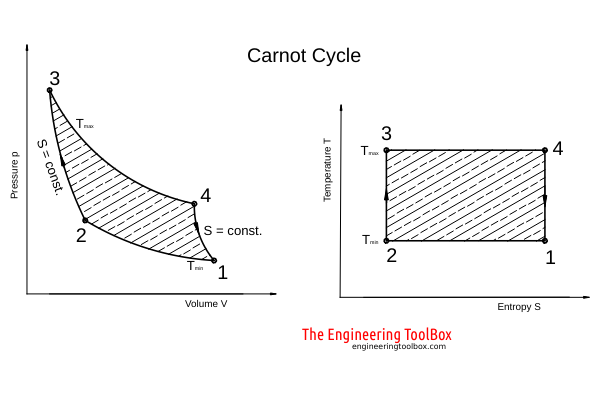
\includegraphics[width=0.5\textwidth]{Foto's-Figuren/carnot_cycle.png}
    \caption{\tiny \copyright{(The Engineering ToolBox, 2008). Carnot Cycle Efficiency. [online] Available at: \url{https://www.engineeringtoolbox.com/carnot-efficiency-d_1047.html} [Accessed 14 May 2026].}}
    \label{Fig:carnot-cycl}
\end{figure}
\begin{derivation}
    Voor een ideaal gas geldt:
    \[\dbar Q = C_V dT + PdV\]
    We passen dit toe op de isotherm \( 1 \to 2 \):
    \[
    Q = \int_{V_1}^{V_2} P dV = nRT \ln\left(\frac{V_2}{V_1}\right) \qquad (T = cst)
    \]
    En op de isotherm \( 3 \to 4 \):
    \[Q' = \int_{V_3}^{V_4} P dV = nRT' \ln\left(\frac{V_4}{V_3}\right) \qquad (T' = cst)\]
    De verhouding geeft ons:
    \[\frac{Q}{Q'} = \frac{T}{T'} \frac{\ln\left(\frac{V_2}{V_1}\right)}{\ln\left(\frac{V_4}{V_3}\right)}\]
    Maar omdat \(2 \to 3\) en \(1 \to 4\) adiabatische processen zijn, geldt:
    \[C_VdT = -PdV = -\frac{nRT}{V}dV\]
    \[\implies \frac{1}{nR}\int_{T'}^{T} \frac{dT}{T} = \ln \frac{V_2}{V_3}\]
    en
    \[\frac{1}{nR}\int_{T}^{T'} \frac{dT}{T} = \ln \frac{V_1}{V_4}\]
    Hieruit volgt dat:
    \[\ln\frac{V_2}{V_3} = \ln\frac{V_1}{V_4} \implies \frac{V_2}{V_3} = \frac{V_1}{V_4} 
    \implies \frac{V_2}{V_1} = \frac{V_4}{V_3 }\]
    Pluggen we dit terug in de verhouding van \(Q\) en \(Q'\) van de kelvin temperatuur in \eqref{eq:Kelvintemp}, dan vinden we:
    \[\frac{Q}{Q'} = \frac{T}{T'}\]
    Wat precies de verhouding is van de Kelvintemperaturen \(T_k\) en \(T_k'\) zoals we net hebben gedefinieerd.
    Als we \(T_k'\) en \(T'\) gelijk stellen aan 273,15 K dan:
    \[T = T_k\]
    De Kelvintemperatuur (onafhankelijk van de stof) is dus gelijk aan de ideale gastemperatuur (afhankelijk van de stof).
    \qed
\end{derivation}
    
\section{Entropie}

\subsection{Begrip Entropie}

Onze Kelvinschaal is zo gekozen zodat:
\[
\frac{T}{T'} = \frac{Q}{Q'} = \frac{\phi(T_e)}{\phi(T'_e)}
\]

Waardoor \(T = k \phi (T_e)\) met k een arbitraire constante... Of toch niet? 

Herinner u de warmte-overdracht van twee nabij gelegen RA-oppervlakken?
\[
\dbar Q = \phi (T_e) f(\sigma) d\sigma
\]
\[
\implies \dbar Q = \frac{T}{k} f(\sigma) d\sigma 
\]
\[\implies \frac{\dbar Q}{T} = \frac{1}{k} f(\sigma) d\sigma \]

Nu is het rechterlid een differentiaal van een functie van de toestand, namelijk \(S\), die we \textbf{entropie} noemen.
\[ \frac{\dbar Q_{rev}}{T} = dS\]

Bij een eindige verandering van toestand kunnen we dit integreren:
\[\int_{i}^{f} \frac{\dbar Q_{rev}}{T} = \int_{i}^{f} dS = S_f - S_i\]

Absolute entropie is niet gedefinieerd, maar veranderingen in entropie wel. We kunnen dus enkel \(\Delta S\) bepalen, niet \(S\) zelf.

Voor een reversibel proces geldt:
\[d S = \oint_{\text{reversibel}}
 \frac{\dbar Q_{rev}}{T} = 0\]

 Dit is het Clausius-theorema dat werd afgeleid uit de Carnot-cyclus.

\subsection{Entropie Ideaal Gas}

Herinner u voor een ideaal gas is de eerste hoofdwet:
\[\dbar Q = C_P dT - P dV\]
\[\implies \frac{\dbar Q}{T} = \frac{C_P}{T} dT - \frac{P}{T} dV\]
\[\implies \Delta S = \int_{T_1}^{T} \frac{C_P}{T} dT - \int_{V_1}^{V} \frac{P}{T} dV\]
Als \(C_P = cst\):
\[ S-S_1 = C_P \ln \left(\frac{T}{T_1}\right) - nR \ln \left(\frac{V}{V_1}\right)\]
\[S = C_P \ln T-nR \ln V -C_P \ln T_1 + nR\ln V_1 + S_1 = C_P\ln T-nR\ln V +S_0 \]

\[\boxed{S = C_P\ln T-nR\ln V + S_0} \qquad (C_P = cst)\]


Ook geldt:
\[\dbar Q = C_V dT + P dV\]

\[S = \int_{T_1}^{T} \frac{C_V}{T} dT + nR \int_{V_1}^{V} \frac{dV}{V}\]

Als \(C_V = cst\):
\[\boxed{S = C_V \ln T + nR \ln V + S_0} \qquad (C_V = cst)\]

\subsection{TS-Diagrammen}

Zoals we eerder al een wilde encounter hadden met een TS-diagram de Carnot-cyclus zullen we hier nu verder op ingaan.

\begin{figure}
    \centering
    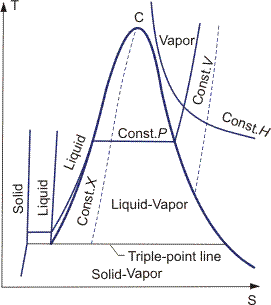
\includegraphics[width=0.8\textwidth]{Foto's-Figuren/TS-Diagram.png}
    \caption{TS-diagram \copyright{Muller-Steinhagen, Hans Michael Gottfried  DOI: 10.1615/AtoZ.t.thermodynamics}}
\end{figure}



\[
\dbar Q_R = TdS \implies Q_R = \int_{i}^{f} TdS
\]



\begin{definition}
    Een \textbf{Isentroop} proces is een reversibel adiabatisch proces, dus waarbij de entropie constant blijft, dus \(dS = 0\).
\end{definition}

De warmtecapaciteiten worden dan:
\[\left(\frac{\dbar Q}{dT}\right)_V = C_V = T\left(\frac{\partial S}{\partial T}\right)_V \qquad (\text{isentroop}, V=cst)\]
en 
\[\left(\frac{\dbar Q}{dT}\right)_P = C_P = T\left(\frac{\partial S}{\partial T}\right)_P \qquad (\text{isentroop}, P=cst)\]

Als \(C_P(T)\) en/of \(C_V(T)\) gekend zijn, kunnen we de entropieverandering van een ideaal gas bepalen:
\[S_f -S_i = \int_{T_1}^{T} \frac{C_V(T)}{T} dT   \qquad (rev, V = cst)\]
\[S_f-S_i = \int_{T_1}^{T} \frac{C_P(T)}{T} dT  \qquad (rev, P = cst)\]

\subsection{De Carnot cyclus}

Misschien kunnen jullie zich de TS-diagram van figuur \ref{Fig:carnot-cycl} nog herinneren. 

\begin{definition}
    De Carnot-cyclus is een reversibele machine werkend tussen slechts twee warmtereservoirs.
\end{definition}

Een warmte-overdracht bij de Carnot-cyclus tussen twee RA-oppervlakken geeft:
\[\frac{Q_H}{T_H} = \frac{Q_K}{T_K}\]
\[\implies \frac{Q_H}{Q_K} = \frac{T_H}{T_K}\]
Waaruit het rendement:
\[\eta = 1 - \frac{Q_K}{Q_H} = 1 - \frac{T_K}{T_H}\] 

Dus
\[
\eta_{\text{Carnot}} = 1 - \frac{T_K}{T_H}
\]

Een rendement van 100\% is alleen mogelijk als \(T_K = 0\) K, wat onmogelijk is volgens de derde hoofdwet van de thermodynamica. Daarom is een rendement van 100\% onbereikbaar.

\begin{postulate}
    Voor elk reversibel proces blijft de entropie van het universum constant. 
\end{postulate}

\subsection{Entropie en Irreversibiliteit}

\begin{definition}[Irreversibel Proces]
    Een proces is irreversibel als het niet mogelijk is om het proces in omgekeerde richting te laten verlopen zonder veranderingen in de omgeving.
    Zo een proces kan beschreven worden als:
    \[\Delta S_{sys} = S_f-S_i = \int_{i, \text{Rev}}^{f} \frac{\dbar Q}{T}\]
    De integratie gebeurt hier langs een (vervangend) reversibel pad (maar niet langs het oorspronkelijke pad), maar het proces zelf is irreversibel.
\end{definition}

\subsubsection{Uitwendige Mechanische Irreversibiliteit}

De irreversibel verrichte arbeid kunnen we vervangen door een reversibel proces met reversibele isobare overdracht van warmte, zodat we de entropieverandering kunnen bepalen:
\[\Delta S_{sys} = \int_{T_i, \text{Rev}}^{T_f} \frac{\dbar Q}{T} = \int_{T_i, \text{Rev}}^{T_f} C_P\frac{dT}{T}\]
Als \(C_P\) constant is:
\[\Delta S_{sys} = C_P \ln \left(\frac{T_f}{T_i}\right) \qquad (C_P = cst)\]


\subsubsection{Interne Mechanische Irreversibiliteit}

Vb: een isotherm proces van een ideaal gas met dus \(\dbar Q_R = PdV\)
\[\implies \frac{\dbar Q_R}{T} = nR\frac{dV}{V}\]

Entropieverandering:
\[\Delta S_{sys} = \int_{Rev,V_i}^{V_f} nR\frac{dV}{V} = nR \ln \left(\frac{V_f}{V_i}\right)\]

\subsubsection{Externe Thermische Irreversibiliteit}
\[\Delta S_{\text{univ}} = \sum \Delta S = \frac{Q}{T_K} - \frac{Q}{T_H}\]

\subsubsection{Chemisch Irreversibel Proces}

Vb: diffusie twee verschillende inerte gassen:

stel \(\frac{V_i}{n} = 1\) en \(\frac{V_f}{n} = 2\), dan is de entropieverandering:
\[\Delta S_{sys} =  R \ln \left(\frac{2}{1}\right) + R \ln \left(\frac{2}{1}\right) = 2R \ln 2\]

Niet zo een belangrijk voorbeeld denk ik \(\dots\)

\subsection{Entropietoename Universum}

Entropie in het universum neemt steeds toe (tot het concept tijd niet meer bestaat \(\dots\))

\begin{proof}[Entropieprincipe]
    Het is voldoende ons te beperken tot adiabatische processen.

    We starten in ons systeem met coördinaten \(T, X\) en \(X'\) op punt \(i\) en eindigen op punt \(f\). 
    We kunnen nu een irreversibel pad vinden van \(i \to f\): 
    \[
    \Delta S = S_f - S_i 
    \]
    en een irreversibel adiabatisch proces van \(f \to k\) zodat de temperatuur \(T'\) wordt van een willekeurig gekozen reservoir.

    Het systeem wordt nu in contact gebracht met dit reservoir, er wordt een reversibel isotherm proces van \(k \to j\) tot ze dezelfde entropie hebben als in punt \(i\).

    Nu gaan we van dit punt terug \(j\) terug naar \(i\) via een reversibel adiabatisch proces.

    De twee processen \(i \to f\) en \(j \to k\) brengen een entropieverandering met zich mee, en de nette entropieverandering van een cyclus is \(0\), dus:

    \[
    (S_f-S_i) + (S_j- S_k) = \Delta S + S_j - S_k = 0
     \implies \Delta S = S_k - S_j
    \]
    De enige warmte-overdracht gebeurt tussen \(k\) en \(j\), en aangezien \(T' > T\) (omdat \(T'\) van een reservoir is), zal er warmte van \(k \to j\) stromen:

    \[
    Q_R = T' (S_j-S_k)
    \]

    De hoeveelheid arbeid verricht is:

    \[
    W_{net} = Q_R
    \]

    Volgens de tweede wet kan kan er geen warmte in het systeem gebracht zijn.
    \footnote{Anders zouden we een machine hebben die werkt tussen een reservoir en een systeem, en die alleen warmte onttrekt aan het reservoir en arbeid levert, wat onmogelijk is volgens de tweede wet.}

    Dus \(Q_R<0\):

    \[
    T'(S_j-S_k) \leq 0 
    \]
    \[
    \implies \Delta S = S_k - S_j \geq 0
    \]

    We kunnen nu veronderstellen dat ons eerste irreversibel adiabatisch proces van \(i \to f\) zou verlopen zonder dat er een entropieverandering zou optreden, dus \(\Delta S = 0\).
    Doordat \(\implies \Delta Q = 0 \), dan zal ook \(W_{net} = 0\) en is er geen toestandsverandering (systeem is terug in punt \(i\)).
    Maar dit betekend dat het proces reversibel is, wat in tegenspraak is met onze aanname dat het proces irreversibel is.

    Dus de entropieverandering kan niet nul zijn, en moet dus positief zijn.
\end{proof}

\begin{postulate}
    De entropieverandeiring van een systeem en zijn omgeving is altijd positief en nadert slechts naar 0 als de processen naar reversibiliteit naderen.
\end{postulate} 

\subsection{Entropieprincipe voor Thermische Machines}

Stel we hebben een machine met een arbitraire cyclus die een hoeveelheid warmte \(Q_H\) onttrekt aan een warmtereservoir bij temperatuur \(T_H\) en een hoeveelheid warmte \(Q_K\) afgeeft aan een koudreservoir bij temperatuur \(T_K\).

De netto entropieverandering van het universum is:
\[\Delta S_{\text{univ}} = \frac{Q_K}{T_K} - \frac{Q_H}{T_H} \geq 0\]

Na het leveren van arbeid \(W\) aan de omgeving, zal er een hoeveelheid warmte \(Q_H - W\) onttrokken worden aan het warmtereservoir, en een hoeveelheid warmte \(Q_K = Q_H - W\) afgegeven worden aan het koudreservoir:
\[\Delta S_{\text{univ}} = \frac{Q_H - W}{T_K} - \frac{Q_H}{T_H} \geq 0\] 

\[\implies W \leq Q_H \left(1 - \frac{T_K}{T_H}\right)\]

Ofwel:
\begin{equation}
\label{eq:W_max}
W_{\text{max}} = Q_H \left(1 - \frac{T_K}{T_H}\right)
\end{equation}  

Het rendement van een machine is gedefinieerd als: 
\[\eta = \frac{W_{\text{max}}}{Q_H} = 1 - \frac{T_K}{T_H}\]

\begin{postulate}
    Het rendement van een machine die werkt tussen twee warmtereservoirs is altijd kleiner dan of gelijk aan het rendement van een Carnot-machine die werkt tussen dezelfde reservoirs.
\end{postulate}

Doen we nu hetzelfde voor een koelmachine:

\[\Delta S_{\text{lichaam}} = S_2 - S_1\]
\[\Delta S_{\text{koelstof}} = 0\]
\[\Delta S_{\text{reservoir}} = \frac{Q}{T_K} - \frac{Q}{T_H}\]

Er volgt:

\[
S_2-S_1 + \frac{Q + W }{T_K} \geq 0
\]

waaruit:

\[
W \geq (S_1-S_2)T_K - Q
\] 

\begin{equation}
\label{eq:W_min}
\implies W_{\text{min}} = (S_1-S_2)T_K - Q
\end{equation}

\subsection{Niet Beschikbare Energie}

Stel je voor we onttrekken een hoeveelheid warmte \(Q\) aan een warmtereservoir bij temperatuur \(T\).
De maximale arbeid gegeven door \eqref{eq:W_max}, dus voor een hoeveelheid warmte \(Q\) onttrokken aan een reservoir,
kan slechts een hoeveelheid arbeid \(W_{\text{max}} = Q \left(1 - \frac{T_0}{T}\right)\) geleverd worden, waarbij \(T_0\) de temperatuur van de omgeving is.

Vb: Irriversibele warmte-overdracht \(Q\) van een reservoir bij \(T_1\) naar een reservoir bij \(T_2\). 
De maximale arbeid die geleverd kan worden is:
\[
W_{\text{max}} 
= 
Q \left(1 - \frac{T_0}{T_1}\right) - Q \left(1 - \frac{T_0}{T_2}\right) 
=
Q \left(\frac{T_0}{T_2} - \frac{T_0}{T_1}\right) 
= 
Q T_0 \left(\frac{1}{T_2} - \frac{1}{T_1}\right)
\]  

\[E = T_0 \Delta S\]

\begin{proof}
    We zullen dit algemener bewijzen voor irriversibele processen. 

    We veronderstellen een systeem dat in contact staat met een warmtereservoir bij temperatuur \(T\) en er een irreversibel proces plaatsvindt van \(i \to j\),
    waardoor de inwendige energie van het systeem verandert van \(U_i\) naar \(U_f\) verhoogt, en er een hoeveelheid warmte \(Q\) onttrokken wordt van systeem naar het reservoir.
    
    Dan zegt de eerste wet:
    \[Q = U_f - U_i - W\]
    en de tweede wet:
    \[0 < (S_f-S_i)_{\text{systeem + directe omgeving}}\]

    Beschouw dat het systeem na het irreversibele proces met een reversibel proces wordt teruggebracht
    naar dezelfde toestand door contact met een reservoir bij temperatuur $T_0$.
    De warmte die bij dit reversibele herstel maximaal uit het systeem kan worden afgevoerd is
    \[Q_{\mathrm{rev}} = T_0\,(S_f - S_i).\]
    Deze energie is niet in arbeid om te zetten. Dit noemen we de niet-beschikbare energie $E$. Dus
    \[E = T_0\,(S_f - S_i).\]
\end{proof}

\begin{postulate}
   Telkens een irreversibel proces plaatsvindt, neemt de niet-beschikbare energie van het systeem toe.
   Deze energie is \(E = T_0 \Delta S\).
\end{postulate}

\begin{postulate}
    De maximale arbeid wordt verkregen wanneer een proces reversibel verloopt.
\end{postulate}

\begin{postulate}[Principe van energiedegradatie]
    Energie heeft een kwaliteit, en deze kwaliteit neemt af bij elke overdracht of conversie.
    De energie gaat niet verloren, maar wordt minder beschikbaar om arbeid te leveren. (nuttige arbeid)
\end{postulate}

\section{Thermodynamische functies en vergelijkingen}

\subsection{Het Smoorproces en Enthalpie}

Het smoorproces, Joule-Kelvin-proces of Joule-Thomson-proces
is een irreversibel proces waarbij een gas van toestand \(i \to j\) gaat.
De verandering in temperatuur tijdens dit proces wordt beschreven door de Joule-Kelvin-coëfficiënt $\mu = \left(\frac{\partial T}{\partial P}\right)_H$.

De eerste hoofdwet:

\[
Q = U_f - U_i - W
\]

met \(Q = 0\)

en
\[
W = - \int_{0}^{V_f} P_fdV - \int_{V_i}^{0} P_i dV
\]

Als de druk constant blijft: \(W = -(P_fV_f - P_iV_i)\)

Dan wordt de eerste hoofdwet:
\[
0 = U_f - U_i + P_fV_f-P_iV_i
\]
\[
\implies U_f + P_fV_f = U_i + P_iV_i
\]
\[
\implies H_f = H_i
\]

De enthalpie.

In het TP-diagram ligt \(\mu\) op het inversiepunt.

\begin{equation}
    \label{eq:enthalpie}
    H = U + PV
\end{equation}

\begin{align*}
dH &= dU + PdV + VdP \\
&= TdS - PdV  + PdV + VdP\\
&= TdS + VdP
\end{align*}

of met \(dU + PdV = dQ\):

\begin{align*}
dH &= dQ + VdP \\
\implies \frac{dH}{dT} &= \frac{dQ}{dT} + V\frac{dP}{dT} \\
\implies \left(\frac{\partial H}{\partial T}\right)_P &= \left(\frac{\partial Q}{\partial T}\right)_P= C_P \\
\end{align*}

\[H_f-H_i = \int_{T_i}^{T_f} C_P dT = Q \qquad (\text{Isobaar})\]

Uit \(dH = TdS + VdP\) volgt:

\[\left(\frac{\partial H}{\partial S}\right)_P = T  \qquad\text{en}\qquad   \left(\frac{\partial H}{\partial P}\right)_S = V\]


Bij een isochoor proces grijpen naar de interne energie \(U\), bij een isobaar proces naar de enthalpie \(H\).

\subsection{De Helmholtzfuncties en Gibbsfuncties}

\begin{definition}
\textbf{Helmholtzfunctie} \(F\) is gedefinieerd als:
\[
F = U - TS
\]
\end{definition}

\begin{align*}
dF &= dU - TdS - SdT \\
&= dQ -PdV - TdS - SdT \\
&= -PdV-SdT \\
\end{align*}

Waaruit:
\[P =-\left(\frac{\partial F}{\partial V}\right)_T \qquad\text{en}\qquad S = -\left(\frac{\partial F}{\partial T}\right)_V \]

Voor een reversibel isotherm proces is \(dQ = TdS\) en dus \(dF = -PdV\).

Voor een reversibel isoterm en isochoor proces is \(dF = 0 \implies F = cst\).


\begin{definition}
\textbf{Gibbsfunctie} \(G\) is gedefinieerd als:
\[
G = H - TS
\]
\end{definition}

\begin{align*}
dG &= dH - TdS - SdT \\
&= TdS + VdP - TdS - SdT \\
&= VdP - SdT \\
\end{align*}

Reversibel isotherm en isobaar proces: \(dG = 0 \implies G = cst\)

Belangrijk resultaat van de gibbs vrije energie:

Op de smeltkromme:
\[G_{\text{vast}} = G_{\text{vloeibaar}} \]
Op de verdampingskromme:
\[G_{\text{vloeibaar}} = G_{\text{damp}} \]
Op de sublimatiekromme:
\[G_{\text{vast}} = G_{\text{damp}} \]
\subsection{De Maxwellbetrekkingen}
\begin{derivation}
\textbf{Maxwellbetrekkingen} zijn afgeleid uit de differentiaalvormen van de thermodynamische functies \(U, H, F, G\) en de eigenschappen van partiële afgeleiden. De vier Maxwellbetrekkingen zijn:
\begin{align*}
\left(\frac{\partial T}{\partial V}\right)_S &= -\left(\frac{\partial P}{\partial S}\right)_V \\
\left(\frac{\partial T}{\partial P}\right)_S &= \left(\frac{\partial V}{\partial S}\right)_P \\
\left(\frac{\partial S}{\partial V}\right)_T &= \left(\frac{\partial P}{\partial T}\right)_V \\
\left(\frac{\partial S}{\partial P}\right)_T &= -\left(\frac{\partial V}{\partial T}\right)_P \\
\end{align*}
\end{derivation}   
Als we totale differentiaalen hebben van de vorm:
\[df = Mdx + Ndy\]
Dan geldt dat:
\[\left(\frac{\partial M}{\partial y}\right)_x = \left(\frac{\partial N}{\partial x}\right)_y\]
\begin{derivation}
\textbf{Afleiding van de Maxwellbetrekkingen} begint met de differentiaalvormen van de thermodynamische functies. Bijvoorbeeld, voor de interne energie \(U\):
\[
dU = TdS - PdV
\]
Hieruit kunnen we de partiële afgeleiden van \(T\) en \(P\) ten opzichte van \(S\) en \(V\) bepalen. Door de symmetrie van de tweede afgeleiden van \(U\) (of een andere thermodynamische functie) te gebruiken, kunnen we de Maxwellbetrekkingen afleiden. Bijvoorbeeld, door de tweede afgeleiden van \(U\) te vergelijken, krijgen we:
\[\left(\frac{\partial T}{\partial V}\right)_S = -\left(\frac{\partial P}{\partial S}\right)_V\]
Op dezelfde manier kunnen we de andere Maxwellbetrekkingen afleiden door de differentiaalvormen van \(H, F, G\) te gebruiken.
\end{derivation}    
\subsection{De TdS-vergelijkingen}


De entropie \(S\) kan worden uitgedrukt als een functie van temperatuur \(T\) en volume \(V\), of als een functie van temperatuur \(T\) en druk \(P\). (of als functie van \(P\) en \(V\) maar dat is minder gebruikelijk)

Dus \(S\) van de volgende vormen aannemen:
\[S = S(T,V)\]
\[S = S(T,P)\]
\[S = S(P,V)\]

Nu kunnen we de TdS vormen afleiden:

\begin{align*}
    S &= S(T,V) \\
    dS &= \left(\frac{\partial S}{\partial T}\right)_V dT + \left(\frac{\partial S}{\partial V}\right)_T dV \\
\end{align*}
Voor een reversibel proces geldt \(dQ = TdS\):
\begin{align*}
    dS &= \frac{dQ}{T} \\
    \implies \dbar Q &= TdS \\
    \dbar Q &= T\left(\frac{\partial S}{\partial T}\right)_V dT + T\left(\frac{\partial S}{\partial V}\right)_T dV \\
\end{align*}
Als V = cst (isochoor proces):
\[\dbar Q = T\left(\frac{\partial S}{\partial T}\right)_V dT \implies C_V = T\left(\frac{\partial S}{\partial T}\right)_V\]

\begin{align*}
    TdS &= T\left(\frac{\partial S}{\partial T}\right)_V dT + T\left(\frac{\partial S}{\partial V}\right)_T dV \\ 
    &= C_V dT + T\left(\frac{\partial S}{\partial V}\right)_T   dV \\
\end{align*}

Met maxwellbetrekking \(\left(\frac{\partial S}{\partial V}\right)_T = \left(\frac{\partial P}{\partial T}\right)_V\) vinden we:

\[\boxed{TdS = C_V dT + T\left(\frac{\partial P}{\partial T}\right)_V dV}\]

Op dezelfde manier kunnen we de TdS-vergelijking voor \(S(T,P)\) en \(S(P,V)\) afleiden.

\begin{align*}
    S &= S(T,P) \\
    dS &= \left(\frac{\partial S}{\partial T}\right)_P dT + \left(\frac{\partial S}{\partial P}\right)_T dP \\
    TdS &= T\left(\frac{\partial S}{\partial T}\right)_P dT + T\left(\frac{\partial S}{\partial P}\right)_T dP \\
\end{align*}

Als \(P = cst\) (isobaar proces):
\[\dbar Q = T\left(\frac{\partial S}{\partial T}\right)_P dT \implies C_P = T\left(\frac{\partial S}{\partial T}\right)_P\]

\[
\boxed{TdS = C_PdT + T\left(\frac{\partial S}{\partial P}\right)_T dP} 
\]

Maxwellbetrekking \(\left(\frac{\partial S}{\partial P}\right)_T = -\left(\frac{\partial V}{\partial T}\right)_P\) geeft:

\[\boxed{TdS = C_PdT - T\left(\frac{\partial V}{\partial T}\right)_P dP}\]



En voor \(S(P,V)\):
\begin{align*}
    S &= S(P,V) \\
    dS &= \left(\frac{\partial S}{\partial P}\right)_V dP + \left(\frac{\partial S}{\partial V}\right)_P dV \\
    TdS &= T\left(\frac{\partial S}{\partial P}\right)_V dP + T\left(\frac{\partial S}{\partial V}\right)_P dV \\
    &= T\left(\frac{\partial S}{\partial T}\right)_V\left(\frac{\partial T}{\partial P}\right)_V dP + T\left(\frac{\partial S}{\partial T}\right)_P \left(\frac{\partial T}{\partial V}\right)_P dV \\
    &= C_V\left(\frac{\partial T}{\partial P}\right)_V dP + C_P \left(\frac{\partial T}{\partial V}\right)_P dV \\
\end{align*}

\subsubsection{Reversibele isotherme drukverandering}

\[TdS = \dbar Q= -T \left(\frac{\partial V}{\partial T}\right)_P dP\]

\[\implies Q= -T \int \left(\frac{\partial V}{\partial T}\right)_P dP\]

Herinner \(\beta = \frac{1}{V}\left(\frac{\partial V}{\partial T}\right)_P\).

Dan:
\[Q = -T \int V \beta dP\]

\[Q = -T \bar{V \beta} (P_f - P_i)\]

\subsubsection{Reversibele adiabatische drukverandering}

Hieronder blijft de entropie constant, dus \(dS = 0\):
\[0 = C_P dT - T \left(\frac{\partial V}{\partial T}\right)_P dP\]

\[\implies  = \frac{T}{C_P}\left(\frac{\partial V}{\partial T}\right)_P d = \frac{TV \beta}{C_P}dP\]

Uit \(dH = TdS + VdP\):

\[
dH = C_P dT - \left[ T\left(\frac{\partial V}{\partial T}\right)_P - V \right] dP
\]
\[
\implies dT = \frac{1}{C_P}\left[ T\left(\frac{\partial V}{\partial T}\right)_P - V \right] dP + \frac{1}{C_P}dH
\]

De Joule-Kelvin-coëfficiënt \(\mu = \left(\frac{\partial T}{\partial P}\right)_H\)

\[\mu = \frac{1}{C_P}\left[ T\left(\frac{\partial V}{\partial T}\right)_P - V \right]\]

Voor een ideaal gas:

\[\mu = \frac{1}{C_P} \left( T\frac{nR}{P} - V \right) = 0\]

\subsubsection{Energievergelijkingen}

\begin{align*}
    dU &= TdS - PdV \\
    \frac{dU}{dV} &= T \frac{d S}{d V}- P \\
\end{align*}

De eerste energievergelijking:
\[
\boxed{\left(\frac{\partial U}{\partial V}\right)_T = T \left(\frac{\partial P}{\partial T}\right)_V - P}
\]
waar we een maxwellbetrekking hebben gebruikt.

\begin{align*}
    dU &= TdS - PdV \\
    \frac{dU}{dP} &= T \frac{d S}{d P}- P \frac{dV}{dP} \\
    \left(\frac{\partial U}{\partial P}\right)_T &= T \left(\frac{\partial S}{\partial P}\right)_T - P \left(\frac{\partial V}{\partial P}\right)_T
\end{align*}

De tweede energievergelijking:
\[
\boxed{\left(\frac{\partial U}{\partial P}\right)_T = -P \left(\frac{\partial V}{\partial P}\right)_T}
\]

\subsubsection{Enthalpievergelijkingen}

\begin{align*}
dH &= TdS + VdP \\
\frac{dH}{dP} &= T \frac{d S}{d P}+ V  \\
\left(\frac{\partial H}{\partial P}\right)_T &= T \left(\frac{\partial S}{\partial P}\right)_T + V 
\end{align*}
De eerste enthalpievergelijking:
\[\boxed{\left(\frac{\partial H}{\partial P}\right)_T = T \left(\frac{\partial S}{\partial P}\right)_T + V}\]

\begin{align*}
    dH &= TdS + VdP \\
    \frac{dH}{dV} &= T \frac{d S}{d V}+ V \frac{dP}{dV} \\
    \left(\frac{\partial H}{\partial V}\right)_T &= T \left(\frac{\partial S}{\partial V}\right)_T + V \left(\frac{\partial P}{\partial V}\right)_T
\end{align*}
De tweede enthalpievergelijking:
\[\boxed{\left(\frac{\partial H}{\partial V}\right)_T = T \left(\frac{\partial S}{\partial V}\right)_T + V \left(\frac{\partial P}{\partial V}\right)_T}\]


\subsection{De Vergelijkingen van de Warmtecapaciteiten}

We stellen de eerste twee TdS-vergelijkingen gelijk aan elkaar:
\[C_V dT + T\left(\frac{\partial P}{\partial T}\right)_V dV = C_PdT - T\left(\frac{\partial V}{\partial T}\right)_P dP\]    
Oplossen naar \(dT\):
\[dT = \frac{T\left(\frac{\partial V}{\partial T}\right)_P }{C_P - C_V}dP + \frac{T\left(\frac{\partial P}{\partial T}\right)_V }{C_P - C_V}dV\]  

Maar \(T=T(P,V)\), dus:
\[dT = \left(\frac{\partial T}{\partial P}\right)_V dP + \left(\frac{\partial T}{\partial V}\right)_P dV\]

We vinden:
\[
\left(\frac{\partial T}{\partial P}\right)_V = \frac{T\left(\frac{\partial V}{\partial T}\right)_P }{C_P - C_V}
\qquad\text{en}\qquad
\left(\frac{\partial T}{\partial V}\right)_P = \frac{T\left(\frac{\partial P}{\partial T}\right)_V }{C_P - C_V}
\]

Beiden geven:
\[
C_P - C_V = T \left(\frac{\partial P}{\partial T}\right)_V \left(\frac{\partial V}{\partial T}\right)_P
\]

Met de eigenschap van de determinant van de Jacobiaan:
\[\left(\frac{\partial P}{\partial T}\right)_V \left(\frac{\partial T}{\partial V}\right)_P \left(\frac{\partial V}{\partial P}\right)_T = -1\] 
vinden we:
\[\boxed{C_P - C_V = -T \left(\frac{\partial P}{\partial T}\right)_V^2 \left(\frac{\partial V}{\partial P}\right)_T}\]  
Dit is blijkbaar één van de belangrijkste vergelijkingen in de thermodynamica, omdat het een relatie geeft tussen de warmtecapaciteiten \(C_P\) en \(C_V\) en de eigenschappen van het systeem zoals uitgedrukt door de partiële afgeleiden van \(P\) en \(V\) ten opzichte van \(T\).

Deze toont aan dat als \(T \to 0 \implies C_P \to C_V\).

Als \(\left(\frac{\partial V}{\partial T}\right)_P = 0 \implies C_P = C_V\). 

En doordat \(\left(\frac{\partial P}{\partial V}\right)_T\) altijd negatief is en \(\left(\frac{\partial V}{\partial T}\right)^2_P\) positief is, volgt dat \(C_P > C_V\) voor alle systemen.


met:
\[\beta = \frac{1}{V} \left(\frac{\partial V}{\partial T}\right)_P\]
en
\[\kappa = -\frac{1}{V} \left(\frac{\partial V}{\partial P}\right)_T\]
vinden we de eerste vorm van de vergelijking van de warmtecapaciteiten:
\[\boxed{C_P - C_V = \frac{TV\beta^2}{\kappa}}\]

De tweede vorm vinden we door de \(TdS\)-vgl te gebruiken bij \(dS = 0\)
\[C_V dT = - T\left(\frac{\partial P}{\partial T}\right)_V dV_S\]
en 
\[C_PdT = T \left(\frac{\partial V}{\partial T}\right)_P dP_S\]

\[\frac{C_P}{C_V} = \frac{T \left(\frac{\partial V}{\partial T}\right)_P}{- T\left(\frac{\partial P}{\partial T}\right)_V} \left(\frac{\partial P}{\partial V}\right)_S = -\frac{\left(\frac{\partial P}{\partial V}\right)_S}{\left(\frac{\partial P}{\partial V}\right)_T}\]

\[\boxed{\frac{C_P}{C_V} = -\frac{\left(\frac{\partial P}{\partial V}\right)_S}{\left(\frac{\partial P}{\partial V}\right)_T}}\]

We definiëren de adiabatische samendrukbaarheid als:
\[\kappa_S = -\frac{1}{V} \left(\frac{\partial V}{\partial P}\right)_T\].
\[\implies \frac{C_P}{C_V} = \frac{\kappa}{\kappa_S}\]

\subsection{Eerste-orde fase-overgang en de vgl van Clapeyron}

Bij veel fase-overgangen blijven de temperatuur en druk constant, maar veranderen de entropie en het volume. Dit is een eerste-orde fase-overgang.

De fractie van een stof \(x\) kan getransoformeerd worden als:
\[S = n_0(1-x)s_i + n_0 x s_f\]
\[V = n_0(1-x)v_i + n_0 x v_f\]
(\(S\) en \(V\) zijn lineaire functies van \(s_i, s_f\) en \(v_i, v_f\))

Bij reversibile fase-overgangen is de latente warmte \(L\) gedefinieerd als:
\[L = T(s_f - s_i)\] 
de overgedragen warmte bij de fase-overgang.

Uit 
\[dG = VdP-SdT\]
volgt:
\[\left(\frac{\partial G}{\partial P}\right)_T = V \qquad\text{en}\qquad -\left(\frac{\partial G}{\partial T}\right)_P = S\]

Omdat \(G\) continu is tijdens een fase-overgang, zijn ook de partiële afgeleiden van \(G\) continu.

De entropie en/of het volume veranderen, of de eerste afgeleiden van de Gibbsfuncties zijn discontinu.

De warmtecapaciteit tijdens een fase-overgang is oneindig groot, omdat er warmte wordt toegevoegd zonder dat de temperatuur verandert.

\(dT=dP=0\):
\[C_P = T\left(\frac{\partial S}{\partial T}\right)_P \to \infty\]
\[\beta = \frac{1}{V} \left(\frac{\partial V}{\partial T}\right)_P \to \infty\]
\[\kappa = -\frac{1}{V} \left(\frac{\partial V}{\partial P}\right)_T \to \infty\]

Als we de tweede TdS-vlg herschrijven:
\[TdS = C_PdT - TV\beta dP\]
en \(dT = 0 = dP\) en \( C_P = \infty \) nemen is deze vergelijking onbepaald.

Als een toestand \(i \to f\) met een reversibel, isobaar en isotherm proces gaat, dan is de eerste TdS-vlg:
\[TdS = C_V dT + T\left(\frac{\partial P}{\partial T}\right)_V dV\]
\[TdS = T\left(\frac{\partial P}{\partial T}\right)_V dV\]

De druk en temperatuur waarbij de overgang gebeurt, voldoen aan \(P = P(T) \neq P(V,T)\) zodat:
\[\left(\frac{\partial P}{\partial T}\right)_V = \frac{dP}{dT}\]
dan:
\[T(S_f-S_i) = T \frac{dP}{dT}(V_f-V_i)\]
\[\implies \frac{dP}{dT} = \frac{L}{T(V_f - V_i)}\]
Dit is de vergelijking van Clapeyron, die de helling van de fase-overgangskromme in het \(P\)-\(T\) diagram beschrijft.

\begin{proof}
    Bij een overgang op het PV-diagram is \(G_i = G_f\)
    zodat bij een kleine verandering in temperatuur en druk ook \(G_i + dG_i = G_f + dG_f\) geldt.
    Bijgevolg is \(dG_i = dG_f\) en dus \(V_idP - S_idT = V_fdP - S_fdT\).
    Oplossen naar \(\frac{dP}{dT}\) geeft de vergelijking van Clapeyron:
    \[\frac{dP}{dT} = \frac{S_f - S_i}{V_f - V_i} = \frac{L}{T(V_f - V_i)}\]
\end{proof}

Het teken van de helling hangt af van of de stof uitzet of krimpt bij de overgang.
Bij een overgang waarbij de stof uitzet, is \(V_f > V_i\) en is de helling positief. Bij een overgang waarbij de stof krimpt, is \(V_f < V_i\) en is de helling negatief.


\subsection{2e-orde Fase-overgangen en de Vergelijking van Ehrenfest}

De eerste afgeleiden naar \(P\) en \(T\) van de Gibbsfunctie zijn continu tijdens een 2e-orde fase-overgang, maar de tweede afgeleiden zijn discontinu.
\[\left(\frac{\partial S}{\partial T}\right)_P ,\qquad \left(\frac{\partial V}{\partial T}\right)_P, \qquad \left(\frac{\partial S}{\partial P}\right)_T, \qquad \left(\frac{\partial V}{\partial P}\right)_T \]
zijn discontinu.

Doordat:
\[C_P = T \left(\frac{\partial S}{\partial T}\right)_P, \qquad \beta = \frac{1}{V} \left(\frac{\partial V}{\partial T}\right)_P \qquad\text{en}\qquad \kappa = -\frac{1}{V} \left(\frac{\partial V}{\partial P}\right)_T \]
zijn ook \(C_P, \beta\) en \(\kappa\) discontinu.

De overgang van supergeleiding naar normaal geleidend is een voorbeeld van een 2e-orde fase-overgang.

De helling is niet meer gegeven door de vergelijking van Clapeyron, maar door de vergelijking van Ehrenfest:
\[TdS = C_P dT - TV\beta dP\]
\[C_{P,i}dT - TV\beta _{i}dP = C_{P,f}dT - TV\beta _{f}dP\]
\[\implies \frac{dP}{dT} = \frac{C_{P,f} - C_{P,i}}{TV(\beta_f - \beta_i)}\]
Dit is de eerste vergelijking van Ehrenfest.

Er is ook een tweede vergelijking van Ehrenfest.
We gebruiken behoud van volume \(V_i = V_f\)
Op een nabijgelegen punt op de overgangskromme geldt:
\[V_i + dV_i = V_f + dV_f\]
\[\implies dV_i = dV_f\]

\[\left(\frac{\partial V_i}{\partial T}\right)_P + \left(\frac{\partial V_{i}}{\partial P}\right)_T 
= 
\left(\frac{\partial V_f}{\partial T}\right)_P + \left(\frac{\partial V_f}{\partial P}\right)_T dP\]
en:
\[\beta_i V_i dT - \kappa_i V_i dP = \beta_f V_f dT - \kappa_f V_f dP\]
\[\implies \frac{dP}{dT} = \frac{\beta_f - \beta_i}{\kappa_f - \kappa_i}\]
Dit is de tweede vergelijking van Ehrenfest.

\begin{definition}[Lambda-transities]
    Een lambda-transitie is een 2e-orde fase-overgang waarbij de warmtecapaciteit \(C_P\) divergeert, maar \(\beta\) en \(\kappa\) niet. De vergelijking van Ehrenfest is dan niet meer geldig, omdat de teller oneindig wordt. 
    \(T, P, G, S \) en \(V\) zijn constant, maar \(C_P, \beta\) en \(\kappa\) zijn oneindig groot.
\end{definition}


\end{document}